\documentclass[12pt,halfline,a4paper]{ouparticle}
\usepackage{amsmath,amssymb}
\usepackage[round]{natbib}
\usepackage{graphicx,rotating}
\usepackage{dsfont}
\usepackage{xspace}
\usepackage{booktabs}
\usepackage{siunitx}

\newcommand{\Est}[1]{\hat{#1}}

\newcommand{\beginsupplement}{%
        \setcounter{table}{0}
        \renewcommand{\thetable}{S\arabic{table}}%
        \setcounter{figure}{0}
        \renewcommand{\thefigure}{S\arabic{figure}}%
     }
\newcommand{\stopsupplement}{%
        \setcounter{table}{0}
        \renewcommand{\thetable}{\arabic{table}}%
        \setcounter{figure}{0}
        \renewcommand{\thefigure}{\arabic{figure}}%
     }

% method names

\newcommand{\stdpopsim}{\texttt{stdpopsim}\xspace}
\newcommand{\dadi}{$\partial a \partial i$\xspace}
\newcommand{\MSMC}{\texttt{MSMC}\xspace}
\newcommand{\smcpp}{\texttt{smc++}\xspace}
\newcommand{\stairwayplot}{\texttt{stairwayplot}\xspace}
\newcommand{\fastsimcoal}{\texttt{fastsimcoal2}\xspace}
\newcommand{\tskit}{\texttt{tskit}\xspace}

\newcommand{\adk}[1]{\textcolor{red}{ADK: #1}}

\usepackage[hidelinks]{hyperref}
\usepackage[blocks]{authblk}
\renewcommand\Affilfont{\small}
\makeatletter
\renewcommand\AB@affilsepx{, \protect\Affilfont}
\makeatother
\usepackage[utf8]{inputenc}

\begin{document}

\title{A community-maintained standard library of population genetic simulations}
% First authors
\author[1,$\star$]{Jeffrey R. Adrion}
\author[2,$\star$]{Christopher B. Cole}
\author[3,$\star$]{Noah Dukler}
\author[1,$\star$]{Jared G. Galloway}
\author[4,$\star$]{Ariella L. Gladstein}
\author[5,$\star$]{Graham Gower}
\author[6,$\star$]{Christopher C. Kyriazis}
\author[7,$\star$]{Aaron P. Ragsdale}
\author[8,$\star$]{Georgia Tsambos}
% Second Authors
\author[9]{Franz Baumdicker}
\author[10]{Jedidiah Carlson}
\author[11]{Reed A. Cartwright}
\author[12]{Arun Durvasula}
\author[13]{Bernard Y. Kim}
\author[14]{Patrick McKenzie}
\author[15]{Philipp W. Messer}
\author[16]{Ekaterina Noskova}
\author[17]{Diego Ortega-Del Vecchyo}
\author[5]{Fernando Racimo}
\author[18]{Travis J. Struck}
%Senior Authors
\author[7,$\dagger$]{Simon Gravel}
\author[18,$\dagger$]{Ryan N. Gutenkunst}
\author[6,$\dagger$]{Kirk E. Lohmeuller}
\author[1,$\dagger$]{Peter L. Ralph}
\author[4,$\dagger$]{Daniel R. Schrider}
\author[3,$\dagger$]{Adam Siepel}
\author[19,$\dagger$,$\aleph$]{Jerome Kelleher}
\author[1,$\dagger$,$\aleph$]{Andrew D. Kern}

\affil[1]{Department of Biology and Institute of Ecology and Evolution, University of Oregon}
\affil[2]{Wellcome Trust Centre for Human Genetics, University of Oxford}
\affil[3]{Simons Center for Quantitative Biology, Cold Spring Harbor Laboratory}
\affil[4]{Department of Genetics, University of North Carolina at Chapel Hill}
\affil[5]{Lundbeck GeoGenetics Centre, Globe Institute, University of Copenhagen}
\affil[6]{Department of Ecology and Evolutionary Biology, University of California, Los Angeles}

\affil[7]{Department of Human Genetics, McGill University}
\affil[8]{Melbourne Integrative Genomics, School of Mathematics and Statistics, University of Melbourne}
\affil[9]{Department of Mathematical Stochastics, University of Freiburg}
\affil[10]{Department of Genome Sciences, University of Washington}
\affil[11]{The Biodesign Institute and The School of Life Sciences, Arizona State University}
\affil[12]{Department of Human Genetics, David Geffen School of Medicine, University of California, Los Angeles}
\affil[13]{Department of Biology, Stanford University}
\affil[14]{Department of Ecology, Evolution, and Environmental Biology, Columbia University}
\affil[15]{Department of Computational Biology, Cornell University}
\affil[16]{Computer Technologies Laboratory, ITMO University}
\affil[17]{International Laboratory for Human Genome Research, National Autonomous University of Mexico}
\affil[18]{Department of Molecular and Cellular Biology, University of Arizona}
\affil[19]{Big Data Institute, Li Ka Shing Centre for Health Information and
Discovery, University of Oxford}
\affil[$\star$]{Denotes shared first authorship, listed alphabetically}
\affil[$\dagger$]{Denotes shared senior authorship, listed alphabetically}
\affil[$\aleph$]{Denotes corresponding authors, listed alphabetically}
% JK: didn't bother with the \texttt stuff for stdpopsim in the abstract as it's nearly
% always dropped in production anyway.

\abstract{The explosion in population genomic data demands ever more complex
modes of analysis, and increasingly these analyses depend on sophisticated simulations.
Recent advances in population genetic simulation have made it possible to
simulate large and complex models, but specifying such models for a particular
simulation engine remains a difficult and error-prone task.
Computational genetics researchers currently re-implement simulation models
independently, leading to duplication of effort and the possibility for error.
Population genetics, as a field, also lacks standard benchmarks by which new tools for inference might
be measured. Here we describe a new resource, \stdpopsim, that attempts to rectify this situation.
\stdpopsim is a community-driven open source project, which provides a standard
catalog of published simulation models from a wide range of organisms
and supports multiple simulation engine backends.
% PopSim assures correctness in our implementations through a mature, community-based quality control pipeline.
We share some examples demonstrating how \stdpopsim
can be used to systematically compare demographic inference methods,
and we encourage an even broader
community of developers to join in the effort to standardize
population genetic methods.}
\date{}

\keywords{Population genetics, Simulation, Inference}

\maketitle


\section*{Introduction}
While population genetics has always used statistical methods to make inferences from data,
the degree of sophistication of the questions, models, data, and computational approaches
used have all increased over the past decade. Currently there exist myriad computational methods
that can infer the histories of populations
\citep{gutenkunst2009inferring,li2011inference,excoffier2013robust,schiffels2014inferring, terhorst2017robust,ragsdale2019models},
the distribution of fitness effects \citep{Boyko:2008cr,kim2017inference,tataru2017inference,Fortier703918,Huang2019,Vecchyo770966},
recombination rates \citep{chan2012genome,lin2013fast,Adrion662247,Barroso2019},
and the extent of positive selection in genome sequence data
\citep{eyre2009estimating, alachiotis2012omegaplus,degiorgio2016sweepfinder2,kern2018diplos,sugden2018localization}.
While these methods have increased our understanding of the
impacts of genetic and evolutionary processes, very little has been done to systematically
benchmark the quality of inferences gleaned from computational population genetics.
As large databases of population genetic variation begin to be used to inform public health procedures,
the accuracy and quality of these inferences is becoming ever more important.
Assessing accuracy in population genetics is challenging in large part because
 ``ground-truth'' in population genetics comes from simulation,
not from empirical observations, and as a field there has been no agreement
on community standards or best practices. The general modus operandi to date has been to
introduce methods that are validated by a set of bespoke simulations produced by individual
groups. Beyond inefficiency from duplicated effort, such a situation leads
to decreased reproducibility and transparency across the entire field.
Here we describe \stdpopsim, a community-driven catalog
of standardized population genetics models spanning a variety of common study organisms.
This resource will empower the field to rigorously evaluate population genetic software,
%and select the best tool for a given task,
thereby substantially increasing the reliability of population genetic inferences.
%DRS: still not in love with this last sentence here, but tried to make it a little less sappy by adding some explanation.
%ADK: made some edits here
%RNG: Removed the sap. :-P Feel free to put it back if you like it better.
%JK: not crazy about it either. Making it shorter helps though?

The degree to which modeling assumptions and choices of data summaries can affect the ultimate results of population genetic inference has been challenging to assess. Yet there
have been several clear examples of different methods yielding fundamentally
different conclusions. For example, Markovian coalescent methods applied to human genomes have
suggested large ancient ($>100,000$ years ago) ancestral population sizes and
bottlenecks that have not been detected by methods based on allele frequency spectra
\citep[see][]{beichman2017comparison}.
These distinct methods differ in how they model, summarize, and optimize fit to
genetic variation data, suggesting that such design choices can greatly affect the
performance of the inference. Furthermore, it is reasonable
to assume generally that specific methods will perform better than others under certain scenarios.
However, because these conditions are typically unknown, empirical researchers
lack principled guidelines for deciding which statistical method is best suited
to accurately answer their particular question. The need for empirical
guidance will only increase as researchers continue to generate more genomic
variation data from non-model taxa and wish to make inferences regarding
demography and selection.

One way to benchmark different methods for statistical inference in population
genetics is to apply the methods to simulated datasets where the true model
parameters are known. Methods that perform well will accurately infer these
parameters and will also provide reasonable estimates of uncertainty of the
estimated parameters. Indeed, simulation studies are a standard ingredient in
most papers proposing new methods in population genetics. However, these
studies often use simulations of the particular models for which the method was designed,
which showcases the novel method rather than rigorously comparing performance to competing methods.
Of course, testing a new method in the situation for which it was designed is an important step,
but more rigorous testing is necessary for tools that are to be widely used in the field.
% Moreover researchers are generally forced to reimplement previously
% inferred scenarios independently, which makes good benchmarking
% a major additional time investment, and can lead to errors.
% Lastly, the degree to which different methods are compared can be quite variable.
Many more researchers in the broader field
use simulations to perform power and other exploratory analyses.
The many steps of implementing a moderately complicated population genetics simulation,
including translating published demographic models into input for a simulator
and obtaining genetic maps,
present a major obstacle, especially to new researchers.

% One reason why simulation studies do not compare the performance of many methods
% across a wide range of situations
% is that simulation studies are challenging to carry out, for several reasons.
% First, while there are many published population genetic models available, their
% parameters are often not easily accessible, usually presented in supplemental
% tables. Translating these parameters into input for a given simulation engine can
% be a time-consuming and error prone process. In addition, papers often present many
% different models, and different authors may choose to select distinct models,
% making comparison difficult. While improvements in simulation software and ever
% faster computers have partially ameliorated this concern, generating the
% simulated datasets can still be a time and computing resource bottleneck.

For these reasons, we have generated a standardized, community-driven resource
for simulating published demographic models from a number of popular study systems.
This resource, which we call \texttt{stdpopsim}, makes running
realistic simulations for population genetic analysis a simple matter of
choosing pre-implemented models from a community-maintained catalog.
The \stdpopsim catalog currently contains five organisms: humans, \emph{P. pygmaeus},
\emph{D.~melanogaster}, \emph{A.~thaliana}, and \emph{E.~coli}. For each
organism the catalog contains details on the physical organization (e.g., chromosome structure)
of their genomes, one or more genetic maps, default population-level parameters (mutation rate,
generation time) and one or more published demographic histories. Through
either a command line interface or a simple Python API, the user can specify which
organism, genetic map, chromosome, and demographic history they are interested in simulating, and the
simulation output from their chosen model is returned.

The software has been developed by the PopSim Consortium using a
distributed open source model, with strong procedures in place
to continue its growth and maintain its quality.
Importantly, we have rigorous quality control methods to ensure implemented models are accurate
and have documented methods for others to contribute new modules.
We invite new collaborators to join our community.
Below we describe the resource and give
examples of how it can be used to benchmark demographic inference methods.

\begin{figure}[t]
\begin{center}
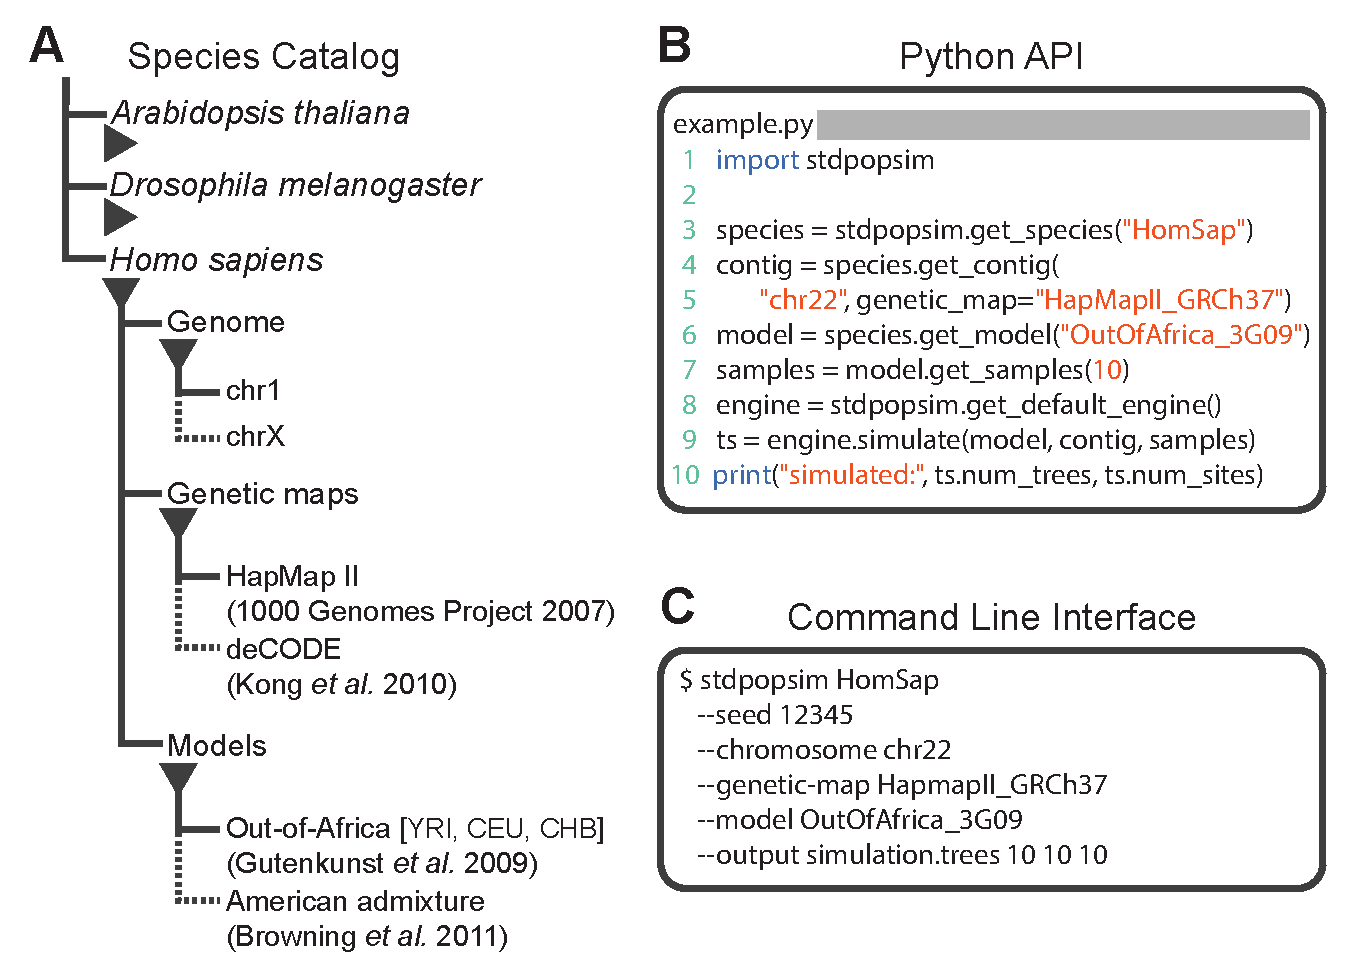
\includegraphics[width=0.5\linewidth]{display_items/Figure1.pdf}
\caption{\textbf{Structure of \stdpopsim}. \textbf{A.} The
hierarchical organization of the PopSim catalog contains all information
within individual species. Information within the species level is shown here
for \emph{Homo sapiens} only. We see that \emph{H. sapiens} is associated
with a default generation time and mutation rate,
a representation of the physical genome, and two genetic maps. Also shown is a
subset of the demographic models currently implemented. \textbf{B.} Caching
and automated download of genetic maps. \textbf{C.} Example code to specify
and simulate models using \stdpopsim via the API (top) or
command-line interface (bottom). \textbf{D.} Simulation output
is a tree sequence file that can
be manipulated and analysed with \tskit.}
\label{fig:cartoon}
\end{center}
\end{figure}

\section*{Results}
\paragraph{The \stdpopsim library}
The first contribution of the PopSim consortium is \stdpopsim, a
community-maintained library of empirical genome data and population genetics simulation
models. Figure \ref{fig:cartoon} shows a graphical
representation of the structure of \stdpopsim. The package centers
on a catalog of species (Fig. \ref{fig:cartoon}A), initially consisting of humans, \emph{P.~abelii},
\emph{D.~melanogaster}, \emph{A.~thaliana}, and \emph{E.~coli}.
% RNG: Abbreviate consistently with introduction
A species definition consists of two key elements.  Firstly, the library defines
some basic information about the species' genome, including information about chromosome
lengths, average mutation rates and so on. We also provide access to detailed
empirical information such as genetic maps, which model observed
heterogeneity in recombination rate along chromosomes. As such maps are often large,
we do not distribute them directly with the software, but make them available
for download in a standard format. When a simulation using such a map is
requested by the user, \stdpopsim will transparently download the map
data into a local cache (\texttt{$\sim$/.local/cache/stdpopsim} by default
on Unix platforms), where it can be quickly retrieved for subsequent
simulations.
In the initial version of \stdpopsim we support
the HapMapII~\citep{international2007second} and
deCODE~\citep{kong2010fine} genetic maps in humans;
the \cite{salome2011recombination} map in \emph{A.~thaliana};
and the \cite{comeron2012many} map in \emph{D.~melanogaster}.
The second key element of a species description
within \stdpopsim is a set of carefully curated population genetic model
descriptions from the literature, which are the basis for accurate simulations
of specific historical scenarios that have influenced present-day patterns of
genetic variation. (See the Methods for a description of the community
development and quality-control process for these models.)

Given the genome data and simulation model descriptions defined within the
library, it is then straightforward to run accurate, standardized simulations
across a range of organisms. \stdpopsim has a Python API and a user-friendly
command line interface, allowing users with minimal experience direct access to
state-of-the-art simulations. Simulations are output in the ``tree sequence''
format \citep{kelleher2016efficient,kelleher2018efficient,kelleher2019inferring}, which
contains complete genealogical information about the simulated samples, is
extremely compact, and can be processed efficiently using the \tskit library
\citep{kelleher2016efficient,kelleher2018efficient}. Currently,
\stdpopsim uses the  \texttt{msprime} coalescent simulator \citep{kelleher2016efficient}
as the default simulation engine. We plan to include other simulation
engines to support scenarios that cannot be modelled under the coalescent framework,
and have already implemented \texttt{SLiM} \citep{haller2019tree,haller2019slim} as
an additional backend.

The \stdpopsim command line interface, by default, outputs citation information
for the models, genetic maps and simulation engines used in any particular run.
We hope that this will encourage users to appropriately acknowledge the
resources used in published work, and encourage authors
of simulation models to contribute to our ongoing community-driven development process.
Together with the \stdpopsim version number and the long-term stable identifiers
for population models and genetic maps,
this citation information will result in well-documented and reproducible
simulation workflows. The individual tree sequence files produced by
\stdpopsim also contain complete provenance information including the command
line arguments, operating system environment and versions of key libraries
used.

\subsection*{The \stdpopsim Catalog}
The current contents of the \stdpopsim catalog are shown in \autoref{tab:catalog}. At the time of
writing, the PopSim Consortium has implemented previously published demographic models for
humans, \emph{Pongo}, \emph{Drosophila}, and \emph{Arabidopsis}.
These range from
simple, single population histories \cite[e.g.,][]{sheehan2016deep},
to complex models which include population splitting, migration, and archaic
admixture \cite[e.g.,][]{ragsdale2019models}.

\renewcommand{\arraystretch}{1.2}
\begin{table}[t]
% Make sure the table is centered even though it's too wide
\makebox[\textwidth][c]{
    \begin{footnotesize}
    \begin{tabular}{lllll}
\hline
\multicolumn{5}{l}{ Homo sapiens (homsap) } \\
\hline
ooa\_3& Three population out-of-Africa& (TODO, 2010)& 10s& 1G \\
ooa\_2& Two population out-of-Africa& (TODO, 2010)& 10s& 1G \\
african& African population& (TODO, 2010)& 10s& 1G \\
america& American admixture& (TODO, 2010)& 10s& 1G \\
ooa\_archaic& Three population out-of-Africa with archaic admixture& (TODO, 2010)& 10s& 1G \\
zigzag& Periodic growth and decline.& (TODO, 2010)& 10s& 1G \\
kamm\_ancient\_eurasia& Multi-population model of ancient Eurasia (Kamm et al. 2019)& (TODO, 2010)& 10s& 1G \\
\hline
\multicolumn{5}{l}{ Drosophila melanogaster (dromel) } \\
\hline
afr\_3epoch& Three epoch African population& (TODO, 2010)& 10s& 1G \\
ooa\_2& Three epoch model for African and European populations& (TODO, 2010)& 10s& 1G \\
\hline
\multicolumn{5}{l}{ Arabidopsis thaliana (aratha) } \\
\hline
fixme& Please give me a descriptive name& (TODO, 2010)& 10s& 1G \\
\hline
\multicolumn{5}{l}{ Escherichia coli (esccol) } \\
\hline
\end{tabular}{lllll}

    \end{footnotesize}
}
\caption{\label{tab:catalog}
Initial set of demographic models in the Catalog and simple benchmarks.
For each model we report the CPU time, maximum memory usage and the
size of the output \tskit file. In each case we simulate 100 samples
drawn from the first population, for the shortest chromosome of that species
and a constant chromosome-specific recombination rate.
The times reported are for a single replicate run on an Intel i5-7600 CPU.
These are not intended to be rigorous benchmarks, and the computing resources
required will vary widely depending on sample sizes, chromosome length,
recombination rates and other factors.
}
\end{table}

At the time of writing, more models of human history have been implemented than for
any other organism. These models include: a simplified version of the \cite{tennessen2012evolution}
model with only the African population specified (expansion from the ancestral
population and recent growth), the three population model of \cite{gutenkunst2009inferring}
which specifies the out-of-Africa bottleneck as well as the subsequent divergence of
the European and Asian populations, the \cite{tennessen2012evolution} two population variant of the
Gutenkunst model which does not include Asian populations, but more explicitly models
recent rapid human population growth, the \cite{browning2018ancestry} admixture model
for American populations which specifies ancestral African, European, and Asian population
components, a three-population out-of-Africa model from \cite{ragsdale2019models}
which includes archaic admixture, a complex model of ancient eurasian admixture from \cite{kamm2019efficiently},
and a synthetic model of oscillating population size from \cite{schiffels2014inferring}.
Together these models
contain features believed to have widespread impacts in real data (e.g. bottlenecks, population growth,
admixture) and are therefore highly pertinent in the context of method development.

For non-human genomes we have have implemented two demographic histories for
\emph{Drosophila melanogaster}, three from \emph{A. thaliana}, an one each from \emph{P. abelii} and \emph{E. coli}.
For \emph{D. melanogaster} we have implemented the three-epoch model estimated by \cite{sheehan2016deep} from
an African sample, as well as the out-of-Africa divergence
and associated bottleneck model of \cite{li2006inferring} which jointly models African
and European populations. For \emph{A. thaliana}, we implemented the
model in \cite{durvasula2017african} inferred using \MSMC. This model includes
a continuous change in population size over time, rather than pre-specified epochs of different
population sizes. We have also implemented a two epoch and a three epoch model estimated from African
samples of \emph{A. thaliana} in \cite{huber2018gene}. For \emph{P. abelii} we have implemented the two 
species divergence model of \cite{locke2011comparative}, which models isolation with migration between \emph{P. abelii}
and \emph{P. pygmaeus}. For \emph{E. coli} we have a simple, large constant population size model implemented.
Beyond organism specific models \stdpopsim also includes a generic piecewise constant size model and 
isolation with migration (IM) model which can be used with any genome and genetic map combination.

\subsection*{Use case: comparing methods of demographic inference}
As an example of the utility of \stdpopsim, we demonstrate how it can be used
to simply and fairly compare popular demographic inference methods.
Although we present comparison of results from several
methods, our aim at this stage is not to provide an exhaustive
evaluation or ranking of these methods. Our hope is instead that future work built upon this resource
will enable more detailed exploration of the strengths and weaknesses of the numerous
inference methods that are available to the population genetics community.

We start by comparing popular methods for estimating
population size histories ($N(t)$) of single populations and subsequently
show simple examples of multi-population inference.
To reproducibly evaluate and compare the performance of inference methods, we developed
\texttt{snakemake} \citep{koster2012snakemake} workflows,
available from \url{https://github.com/popgensims/analysis}.
These workflows allow efficient computing in multicore or cluster environments.

For single-population population size histories, we compared
\MSMC~\citep{schiffels2014inferring}, \smcpp~\citep{terhorst2017robust}, and
\stairwayplot~\citep{liu2015exploring}
 on simulated genomes sampled from a single population,
in a number of the demographic models described above. The pipeline was generalized to
run $R$ replicates with $C$ chromosomes for $n$ samples, for a total of $R \times C$
simulations for each demographic model. After simulation, the pipeline prepares
input files for each of the respective inference methods by grouping all
chromosomes, for each sample, into a single file. For each of the $R$ simulation replicates, this step results in an
input file for each of the
respective inference methods and derived from the same simulated tree sequences.
Each of the inference programs are then run in parallel, followed by plotting of
$N(t)$ estimates from each program.

\begin{figure}
\begin{center}
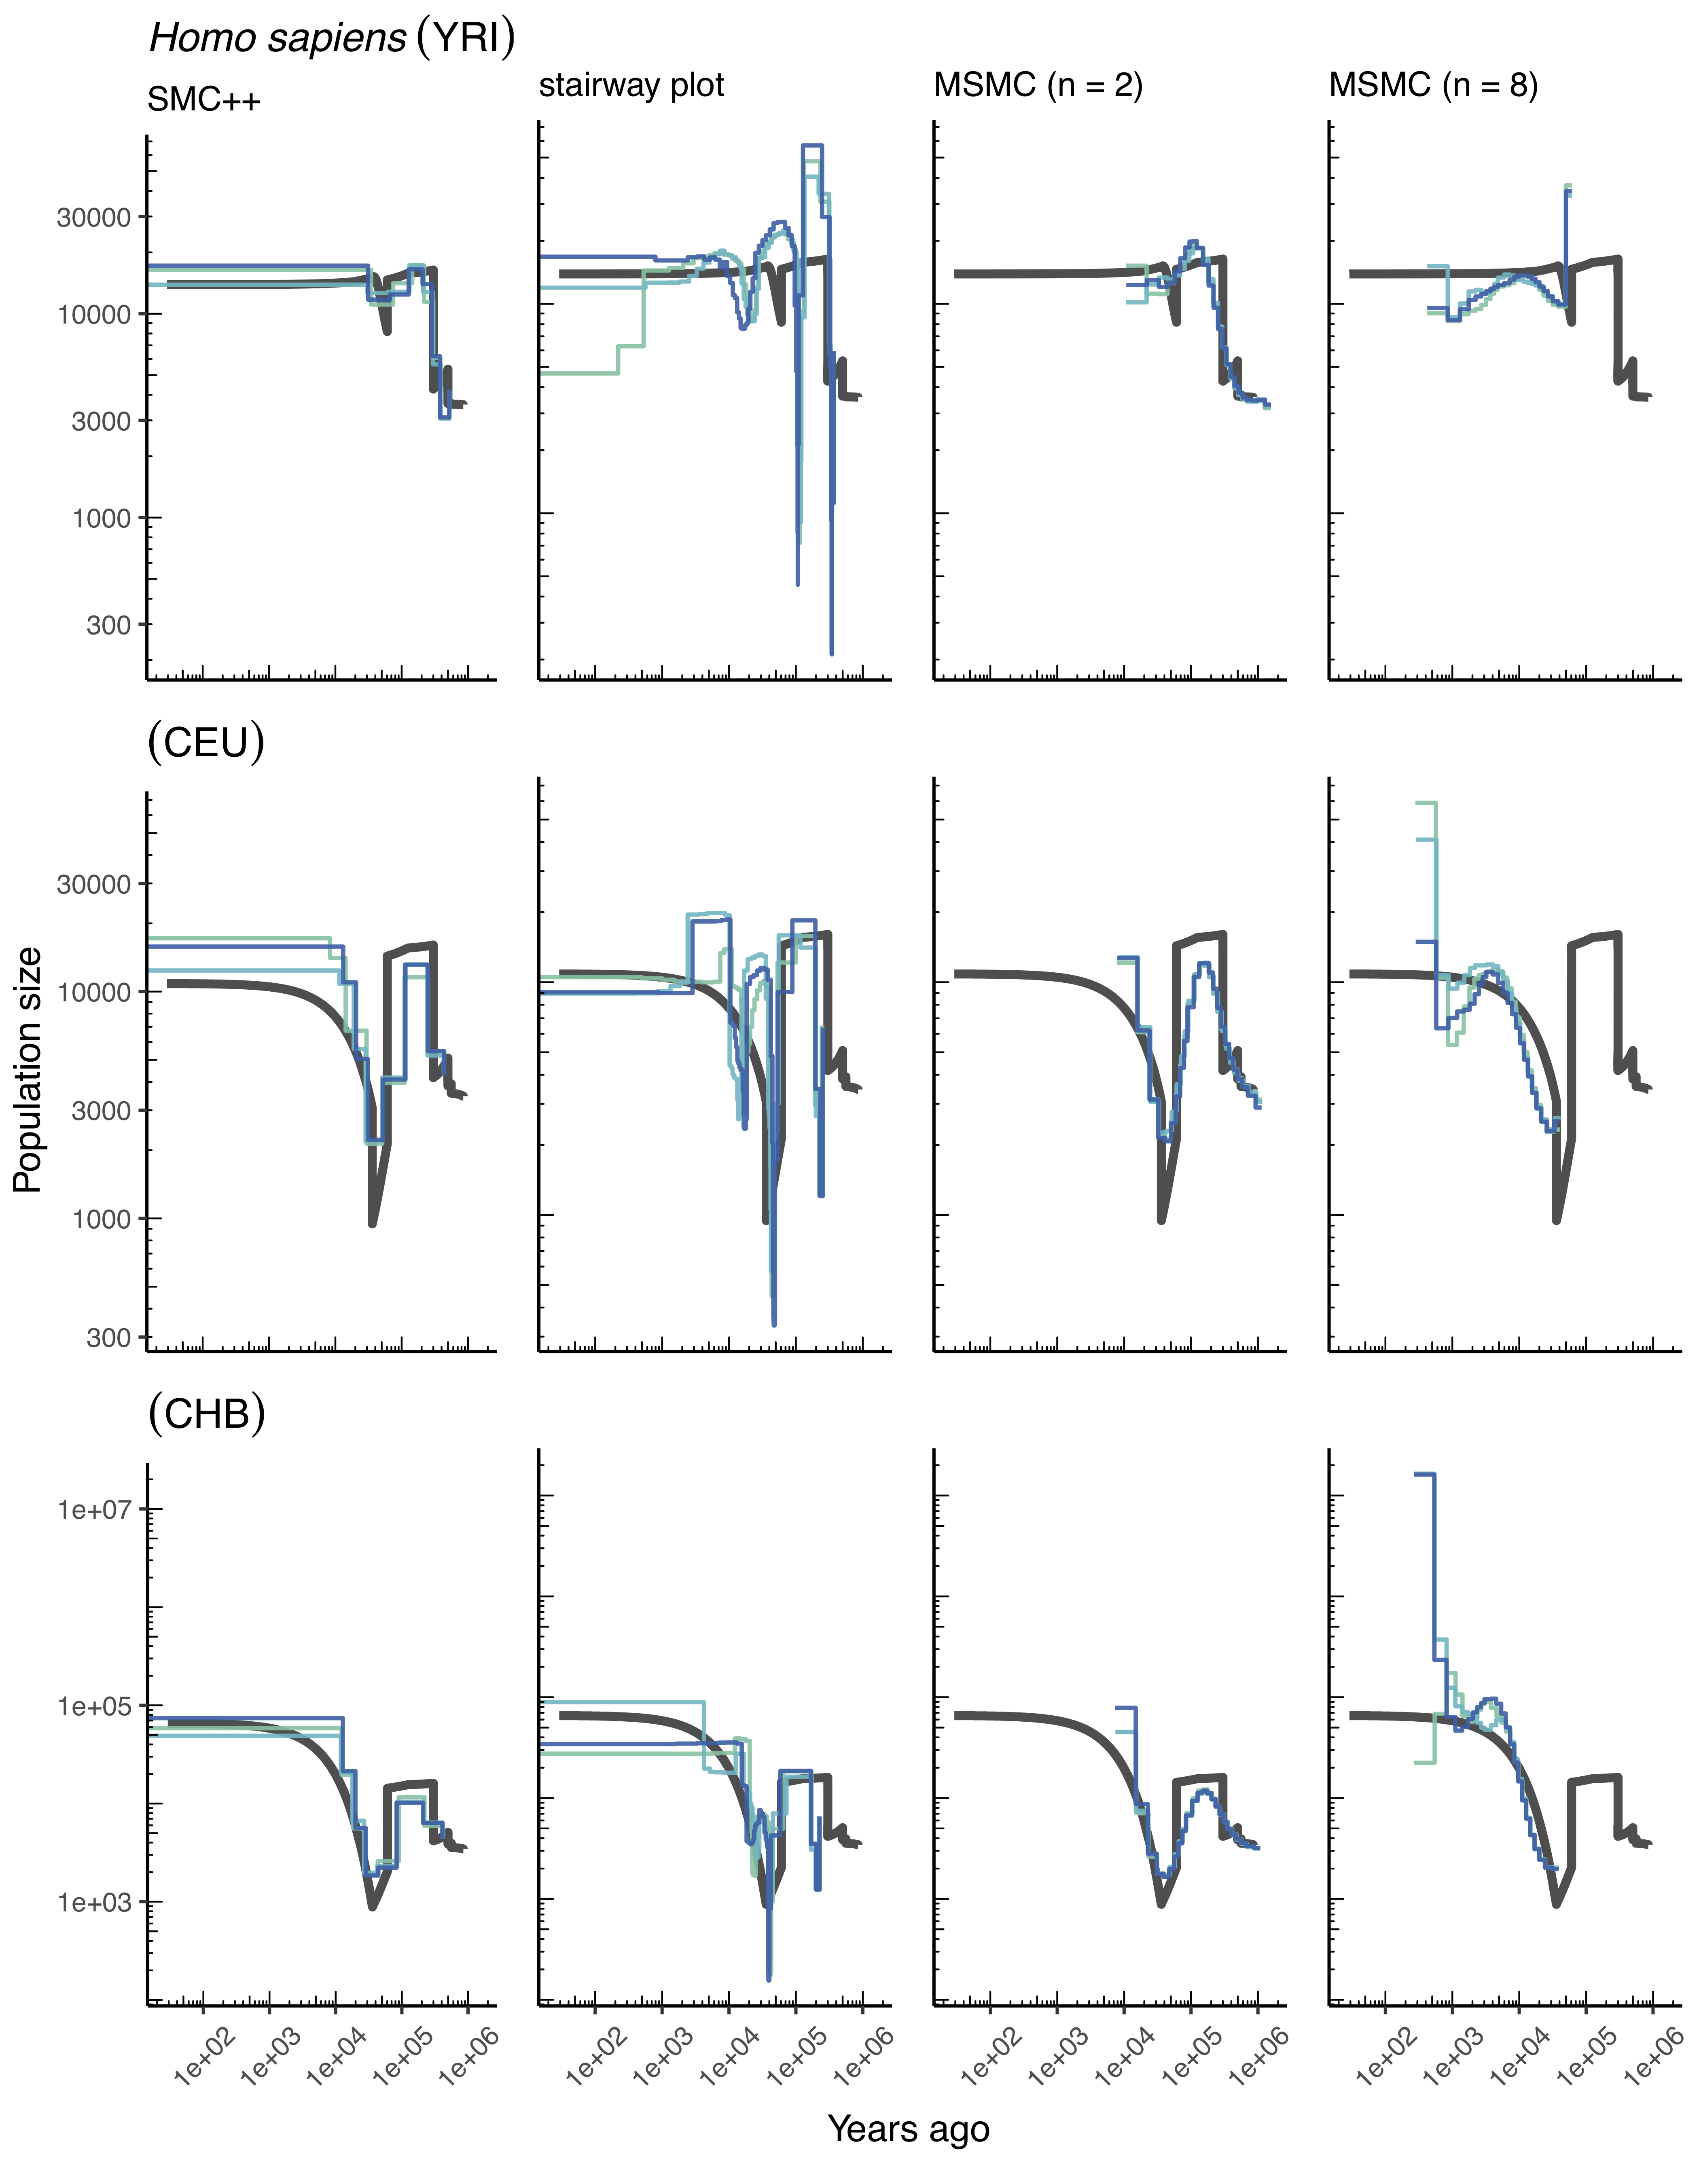
\includegraphics[width=0.8\linewidth]{display_items/homo_sapiens_mask_Ragsdale.png}
\caption{\textbf{Comparing estimates of $N(t)$ in humans}. Here we show estimates of population
size over time ($N(t)$) inferred using 4 different methods: \smcpp, \texttt{stairwayplot}, and
\MSMC with $n=2$ and $n=8$. Data were generated by simulating
replicate human genomes under the \cite{ragsdale2019models} model and using the
HapMapII genetic map~\citep{international2007second}. From top to bottom we show estimates for each
of the three populations in the model (YRI, CEU, and CHB). In shades of blue we show the estimated
$N(t)$ trajectories for each replicate. In black we show the true population size history as inferred
for the rate of coalescence in the demographic model.}
\label{fig:n_t_ragsdale}
\end{center}
\end{figure}


% JK here --- I think it would really help if we described what the models
% were, briefly, rather than saying who inferred them.
In Figure \ref{fig:n_t_ragsdale} we present results from our $N(t)$ analysis pipeline
run on whole genome simulations under under a sophisticated demographic model
and empirical genetic map and a model of human migration out of Africa
that includes archaic admiture \citep{ragsdale2019models}. In each column of this figure
we show inferred $N(t)$ for the three extant populations in the model.
In each row we show comparisons among the methods (note that we compare two differing
sample sizes for \MSMC).
There is no single ``true'' reference for effective population size
because of model misspecification -- the inference methods are fitting a single population model
to data simulated from mulitple populations.
However, many methods work by matching coalescence time distributions,
and a single-population model with varying population size can match any coalescence time distribution
(in which case coalescence rate is the inverse of the effective size).
For this reason, solid black lines do not show historical census sizes,
but rather inverse coalescence rates calculated analytically in \texttt{msprime} (see Appendix).
Blue lines show estimates from each of three replicate whole genome simulations.
While there is variation in accuracy among methods, populations, and individual replicates,
generally the methods are accurate for this model of human history.

\stdpopsim allows us to readily compare these estimates to those drawn from a different
model of human history. In Figure \ref{fig:n_t_gutenkunst} we show estimates of
$N(t)$ from simulations using the same physical and genetic maps, but a different demographic
history that does not include archaic admixture \citep{gutenkunst2009inferring}. Again we see that each
of the methods is capturing relevant parts of the population history, although the
discrepancy between inferred and simulated values varies with $t$. In comparing inferences between the
models it is interesting to note that $N(t)$ estimates for the CHB and CEU
simulated populations are generally better across methods than estimates from the YRI
simulated population.

To see how well methods might do at recovering the population history of a constant sized population,
we can simulate under a human genome architecture and genetic map, but without demography.
We show results of such an
experiment in Figure \ref{fig:n_t_HomSap_constant}. Again we see that all methods
are recovering a modern population size within a factor of two of the truth, however
SMC-based methods, perhaps due to their regularization, tend to learn sinusoidal
patterns of population size even though no change is present.


\begin{figure}
\begin{center}
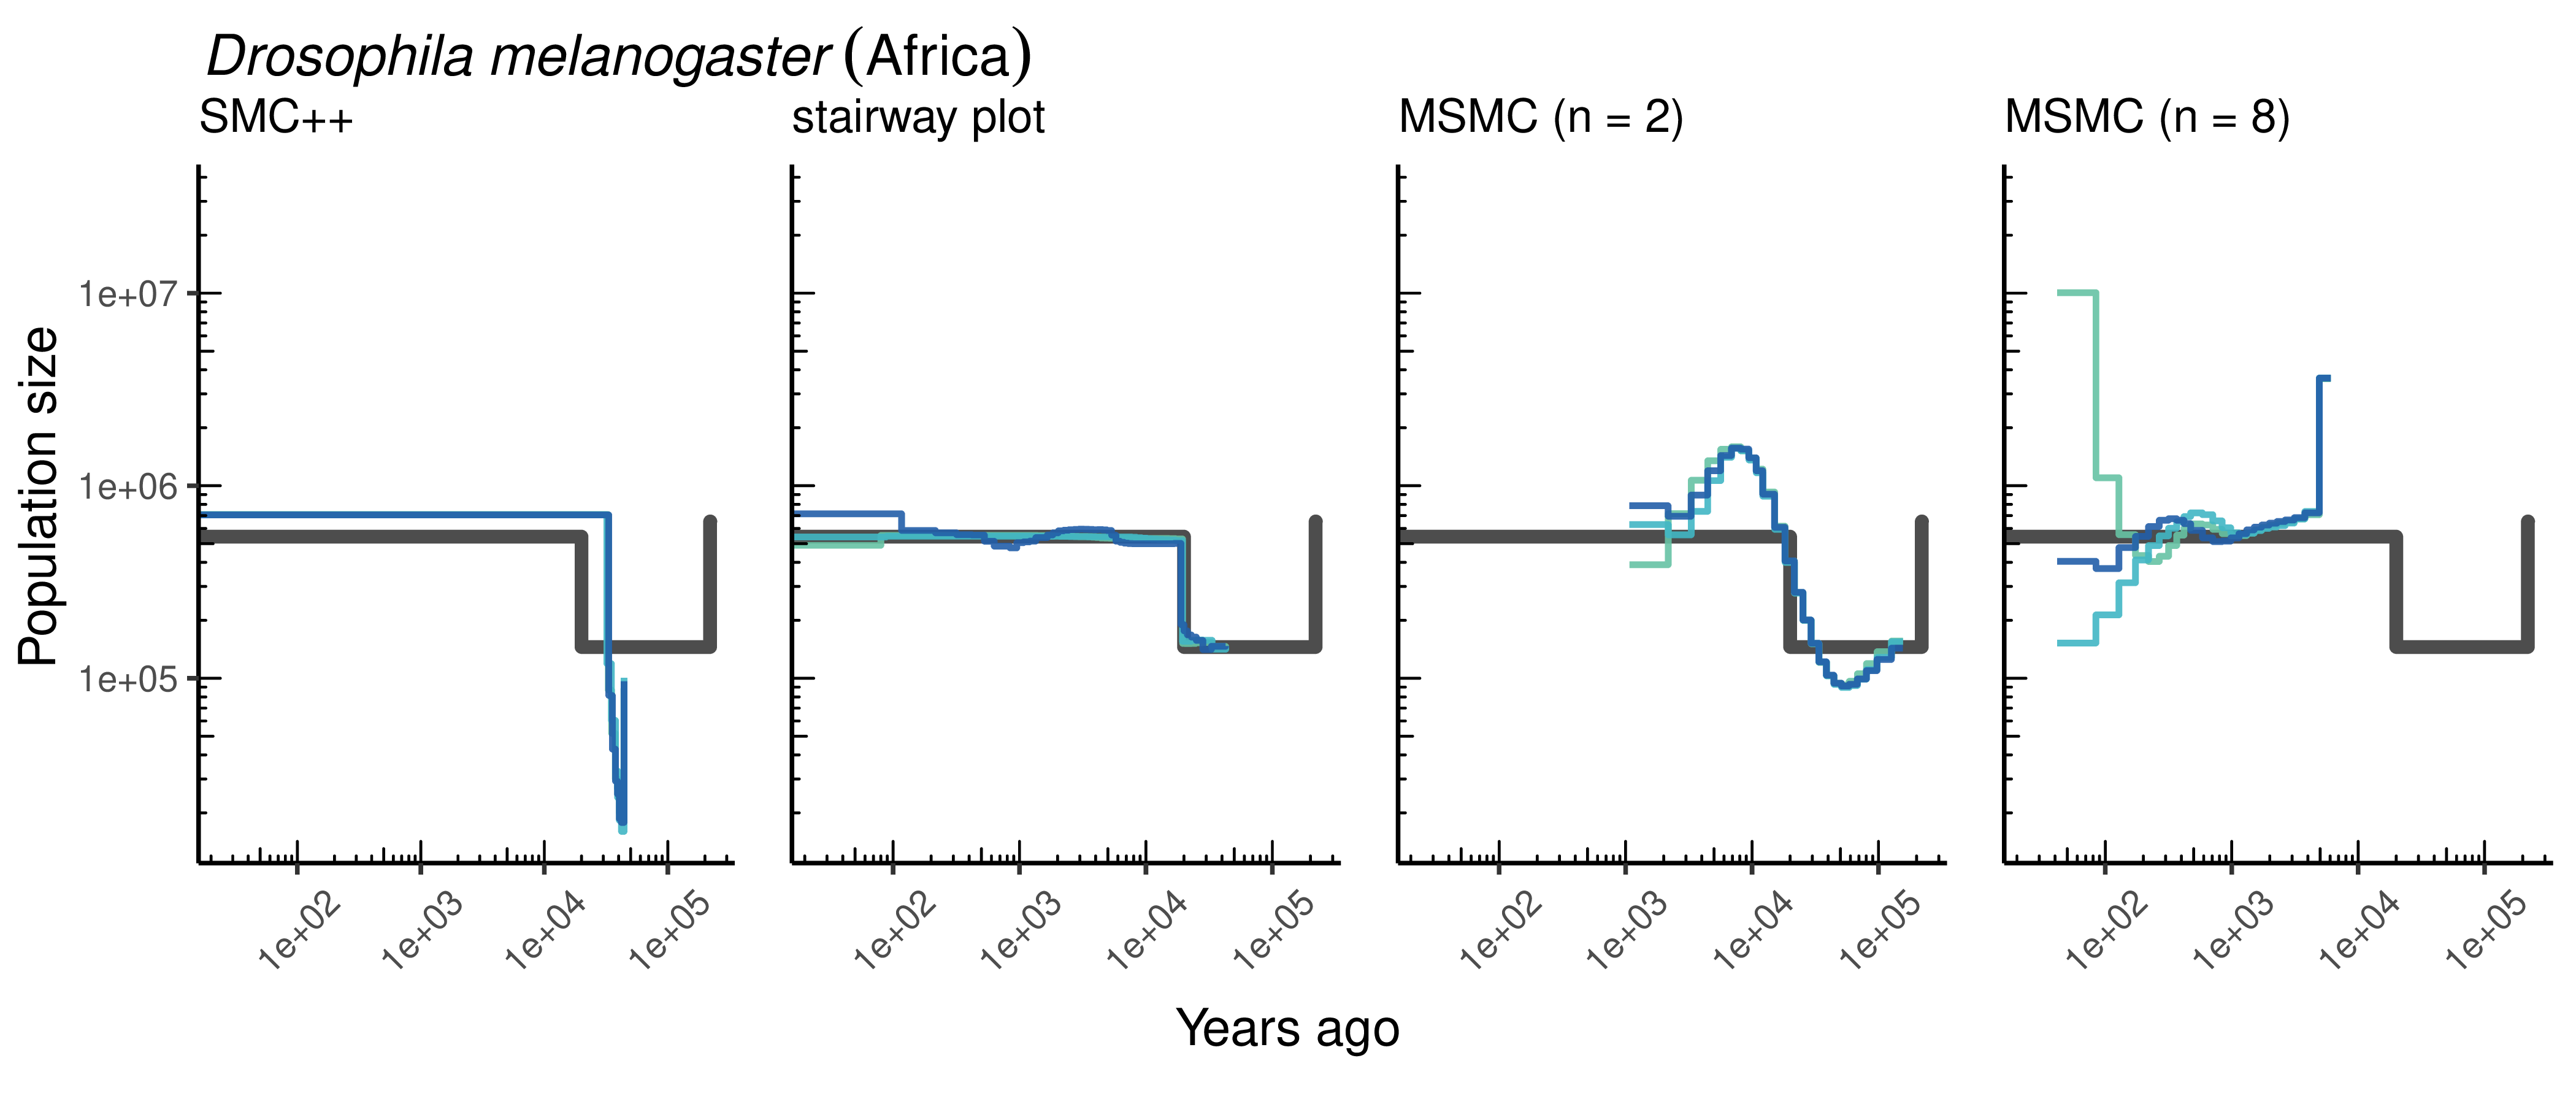
\includegraphics[width=0.8\linewidth]{display_items/d_mel_Sheehan_mask2.png}
\caption{\textbf{Comparing estimates of $N(t)$ in \emph{Drosophila}}. Population
size over time ($N(t)$) estimated from an African population sample. Data were generated by simulating
replicate \emph{D.melanogaster} genomes under the three-epoch \cite{sheehan2016deep} model
with the genetic map inferred in \cite{comeron2012many}. In shades of blue we show the estimated
$N(t)$ trajectories for each replicate. In black we show the true population size history as inferred
for the rate of coalescence in the demographic model.}
\label{fig:n_t_sheehan}
\end{center}
\end{figure}

As most method development for population genetics has been focused on human
data, it is of consequence to ask how such methods might perform in non-human
genomes. Figure \ref{fig:n_t_sheehan} shows parameter estimates from a demographic
model estimated from an African sample of \emph{Drosophila melanogaster} \citep{sheehan2016deep}.
As with humans, we use \stdpopsim to simulate replicate \emph{Drosophila} genomes under
an empirically derived genetic map, and then try to infer back the parameters of the model.
Accuracy is mixed among methods in this setting and generally worse than what we
observe under simulations of the human genome.



\begin{figure}
\begin{center}
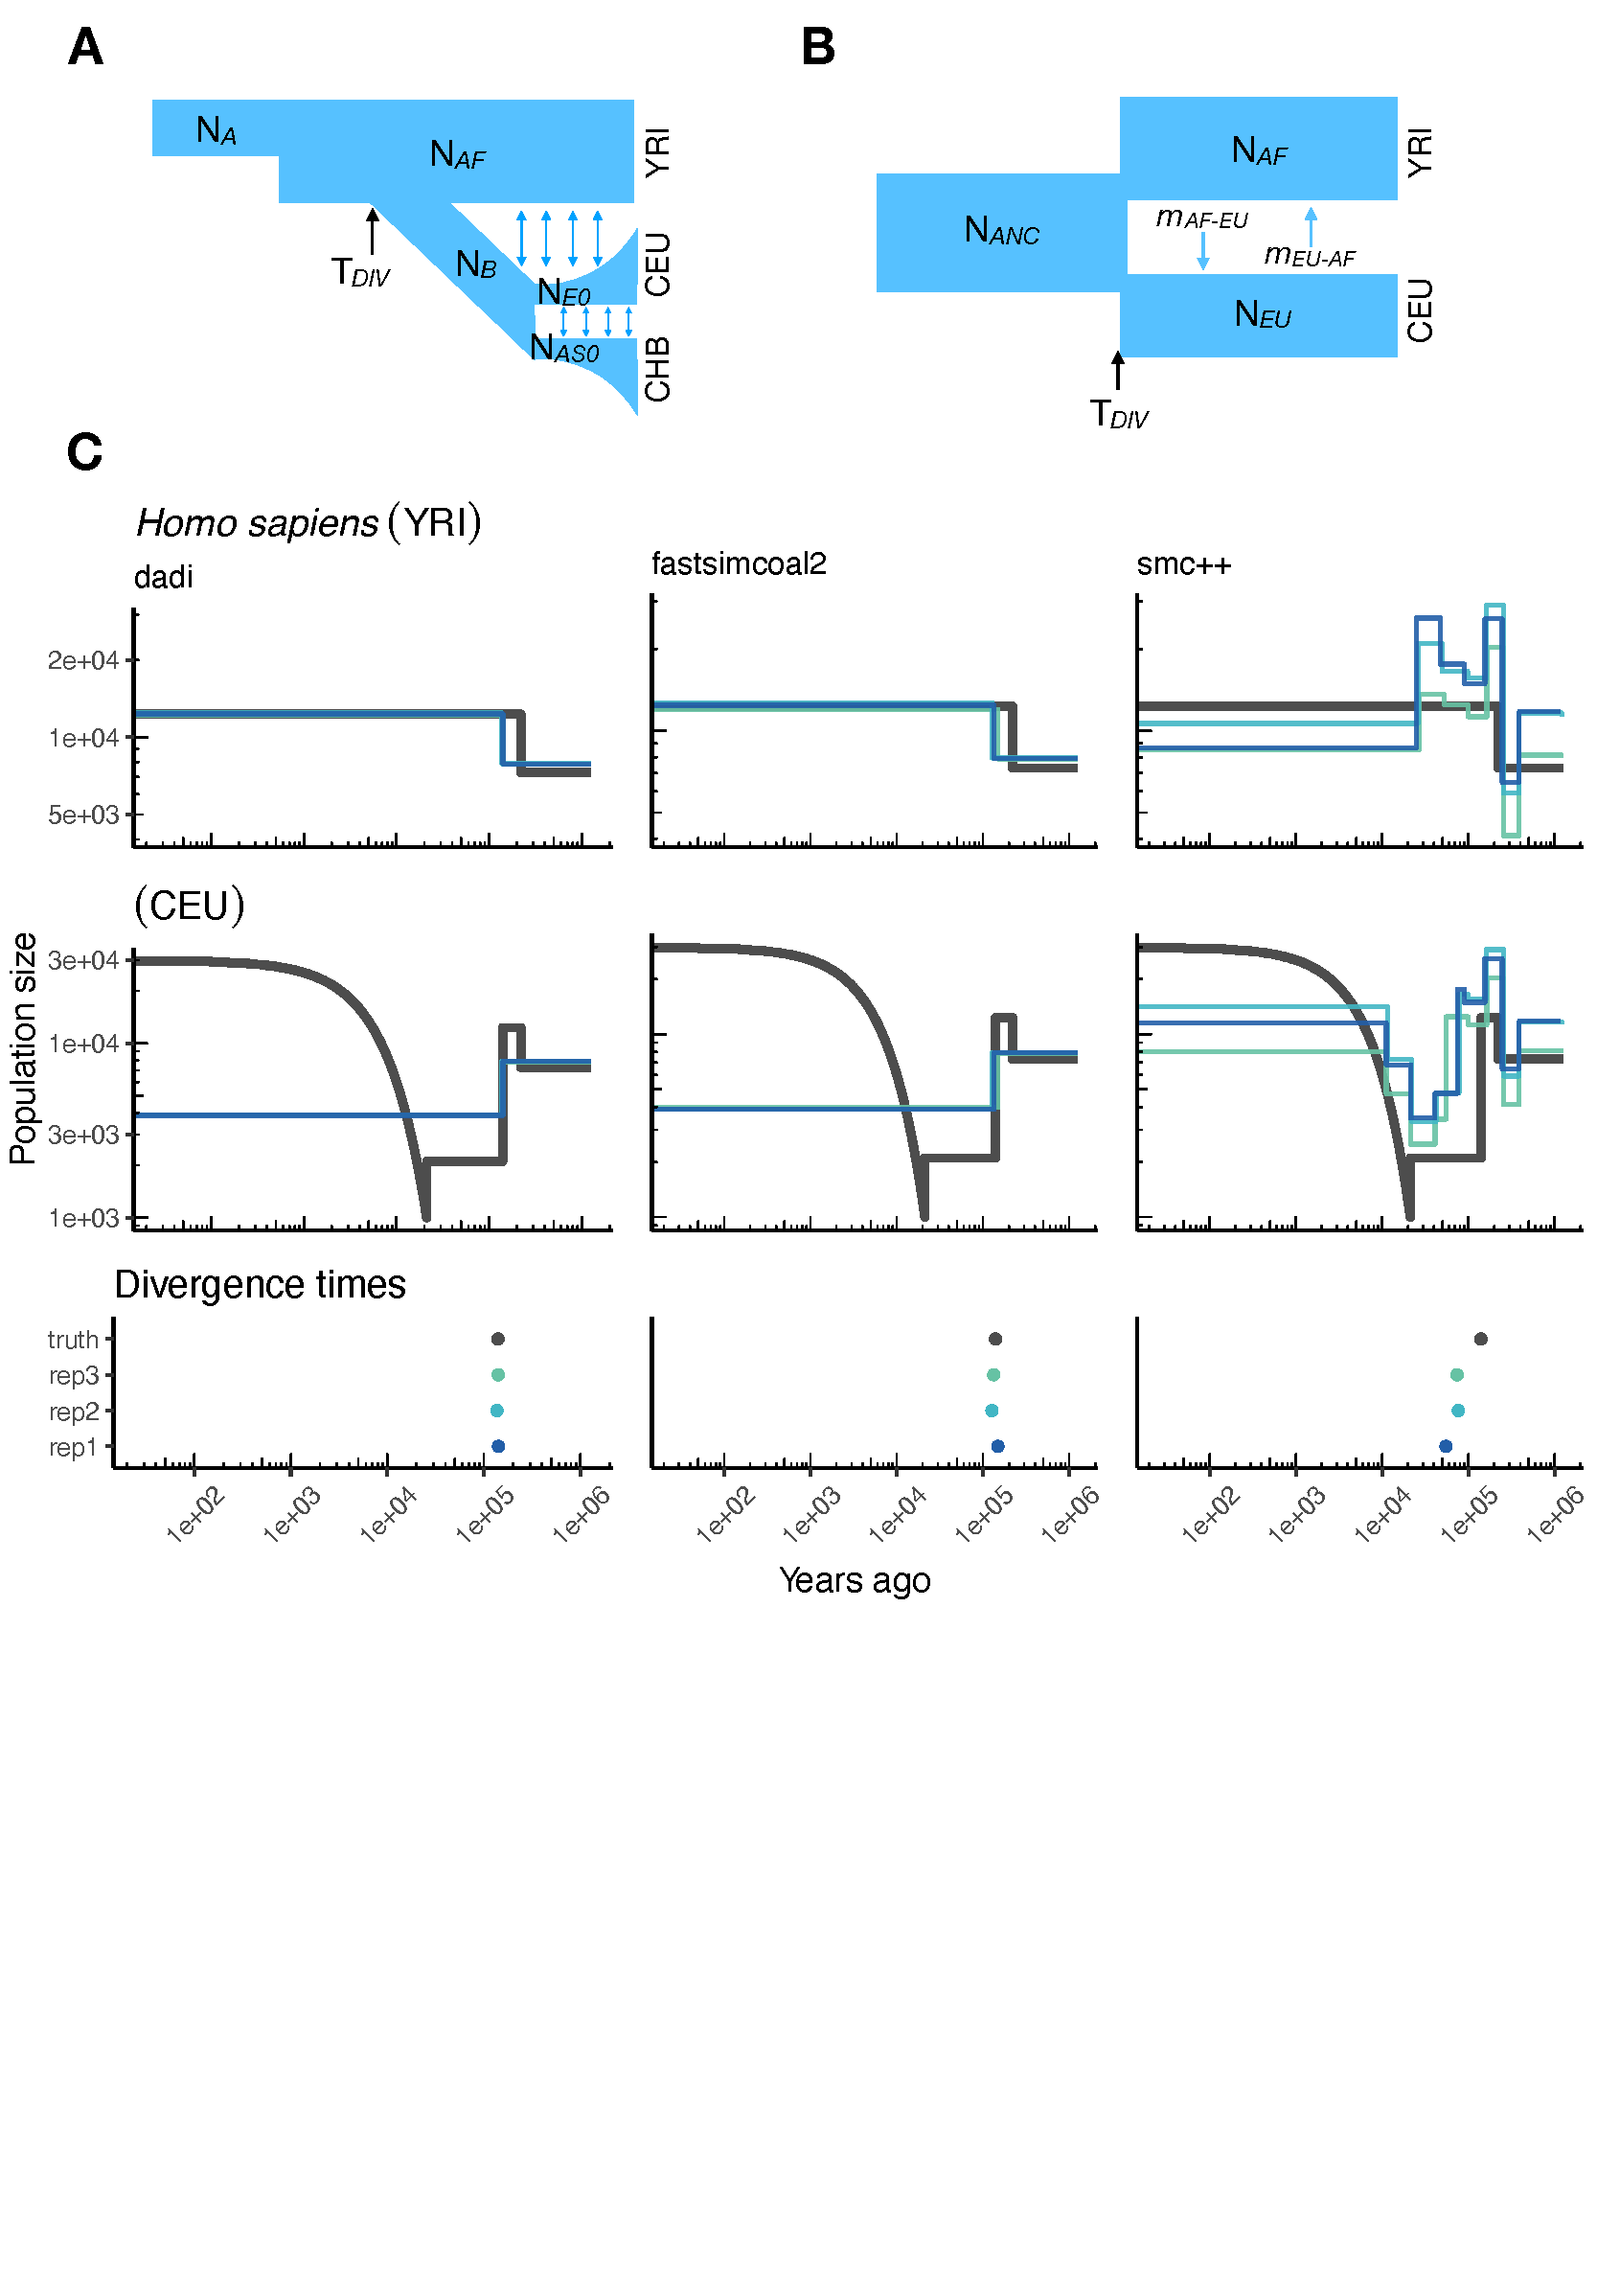
\includegraphics[width=0.7\linewidth]{display_items/homo_sapiens_two_popn_comp.pdf}
\caption{\textbf{Parameters estimated using a multi-population human model}.
Here we show estimates of $N(t)$ inferred using \dadi, \fastsimcoal, or \smcpp.
A) Data were generated by simulating
replicate human genomes under the \cite{gutenkunst2009inferring} model and using the genetic map
inferred in \cite{international2007second}.
B) For \dadi and \fastsimcoal we show parameters inferred
by fitting the depicted IM model, which includes population sizes, migration rates, and a split
time between CEU and YRI samples.
C) Population size estimates for each population (rows)
from \dadi, \fastsimcoal, and \smcpp (columns).
In shades of blue we show $N(t)$ trajectories estimated from each simulation,
and in black the inverse coalescence rates calculated from the true model (see text).
The population split date, $T_{div}$, is shown at
the bottom, with a common X-axis to the population size panels.}
\label{fig:IM_popn_human}
\end{center}
\end{figure}

\paragraph*{Multi-population demographic models}
As \texttt{stdpopsim} implements multi-population demographic models, we also
explored parameter estimation of population divergence parameters. In particular,
we simulated data under multi-population models for humans and \emph{Drosophila}
and then inferred  parameters using \dadi, \fastsimcoal, and \smcpp.
For simplicity, we conducted inference in \dadi and \fastsimcoal by fitting an IM model
with constant population sizes and bi-directional migration \citep{hey2004im}. Our motivation for using
an IM model was to mimic the approach often used on empirical datasets, where a relatively
simple model is fit that may not reflect the true underlying demography.
For human models with more than two-populations (e.g. \cite{gutenkunst2009inferring})
this means that we are inferring parameters for a model which itself does
not match the model from which the data were generated (Figure
\ref{fig:IM_popn_human}A and B).

In Figure \ref{fig:IM_popn_human}C we show estimates of population sizes and divergence
time, for each of the inference methods, using samples drawn from African and European populations
simulated under the \cite{gutenkunst2009inferring} model. Our results highlight many
of the strengths and weaknesses of the different types of methods we used.
For instance, the SFS-based approaches where we fit simple IM models do not capture
recent exponential growth in the CEU population, however do consistently recover the
simulated YRI population size history. Moreover, these approaches allow for estimating
migration rates (Figure \ref{fig:homsap_mig_rates}), also leading to more accurate inference
of divergence times. By contrast, \smcpp is much better at capturing the recent exponential
growth in the CEU population, though the inferred population sizes are in general more
noisy. In addition, the assumption of no migration by \smcpp leads to divergence time
estimates that are consistently underestimated.

Again, we can compare between species and look at the performance of these methods in
the context of a two-population model from \emph{Drosophila melanogaster}. Figure
\ref{fig:two_popn_fly} shows parameter estimates for simulations drawn from
the model of \cite{li2006inferring}, which includes
an ancestral population in Africa, then a population expansion with a population
split and bottleneck into a European population with no post-divergence migration.
Here again, we find that \dadi and \fastsimcoal are more consistent in their inferred
parameters, but ignore the brief population bottleneck in Europe. The inferred
demographic parameters from \smcpp are more noisy, though in some cases are better
able to capture the bottleneck in the Europe population.

Although these results do not represent an exhaustive benchmarking,
we have highlighted some of the strengths and weaknesses of these methods.
Future work should build on these results and undertake more in-depth comparisons
under a wider range of simulated demographic models.

%%%%%%%%%%%%%%%%%%%%%%%%%%%%%%%%%%%%
\section*{Discussion}

Here we have described the first major product from the PopSim Consortium:
the \stdpopsim library. We have founded the Consortium with a number of specific goals in mind:
standardization of simulation within the computational genetics community,
increasing reproducibility and ease of use of complex simulation based results,
community-based development and decision making guiding best practices in population genetics,
and eventual benchmarking of inferential methods.

The \stdpopsim library allows for rigorous
standardization of complex population genetic simulations. Population genetics, as a field,
has yet to coalesce around a set of standards for the crucial task of method
evaluation, which in our field hinges on simulation. In contrast, other fields such as
structural biology \citep{moult1995large} and machine learning \citep{russakovsky2015imagenet} have a long track record
of standardized method testing. We hope that our efforts represent the beginning of what
will prove to be an equally longstanding and valuable tradition in population genetics.

% (ACS) I suggest deleting the following paragraph (commented out below).
% All of the important points are made below (even with some of the same
% phrases, such as "barriers to entry") and I think it is needlessly
% redundant.

%Individual research groups are often in the position of having to independently
%reimplement complex, previously published demographic models.
%Additional layers of realism (e.g., recombination maps) make this especially daunting.
%\stdpopsim aims to lower this barrier
%by creating a quality controlled, easy-to-use, gateway to models and organisms
%that are central to modern research in genetics.

We have illustrated in this paper how \stdpopsim can be used for direct
comparisons of inferential methods on a common set of simulations. Our
benchmarking comparisons have been limited, but nevertheless
reveal some informative features. For
example, at the task of estimating $N(t)$ trajectories for simulated human
populations, we find that the sequence-based methods (\MSMC and \smcpp)
perform somewhat better overall---at least for mid-range values of
$t$---than the site frequency spectrum-based method (\stairwayplot)
(Figures~\ref{fig:n_t_ragsdale} and~\ref{fig:n_t_gutenkunst}), which
tends to over-estimate the sizes of oscillations.  By contrast,
\stairwayplot outperforms the sequence-based methods
on simulations of \textit{D.~melanogaster} populations,
in which linkage disequilibrium is considerably reduced (Figure~\ref{fig:n_t_sheehan}).
In simulations of two human populations
(Figure~\ref{fig:IM_popn_human}), most methods do reasonably well at
reconstructing the YRI history, but struggle with the more complex CEU
history, in large part because of the restriction of constant sizes per
population.  An exception is \smcpp, which does not have the same
restrictions on its inferred history, and as a result does somewhat better
with the CEU history but tends to overfit the YRI history.  The results for
the two-population \textit{D.~melanogaster} case (Figure~\ref{fig:two_popn_fly})
are generally similar.

Altogether, these preliminary experiments highlight
the utility of \stdpopsim for comparing a variety of inference methods on
the same footing, under a variety of different demographic models.
In addition, the ability of \stdpopsim to generate data with and without significant features, such
as a genetic map or population size change (e.g., Figure \ref{fig:n_t_HomSap_constant}), allows
investigation of the failure modes of popular methods.
Moreover the comparison of methods across the various genome organizations, genetic maps,
and demographic histories of different organisms, provides valuable information
about how methods might perform on non-human systems.

Finally, comparison of results across methods or simulation runs
provides an estimate of inference uncertainty, analogous to parametric
bootstrapping,
especially since different methods are likely vulnerable to model misspecification
in different ways.

\stdpopsim is intended to be a fully open, community-developed project.
Our implementations of genome representations and genetic maps for the some of
the most common study systems in computational genetics---humans, \textit{Drosophila},
and \textit{Arabidopsis} (among others)---are only intended to be a starting point for
future development.  In addition to other taxa,
we hope to soon incorporate other common biological processes
such as selection, gene conversion, and mutational heterogeneity.
Researchers are invited to contribute to the resource by adding their
organisms and models of choice. The \stdpopsim resource is
accompanied by clearly documented standard operating procedures that are
intended to minimize barriers to entry for new developers.  In this way, we
expect the resource to expand and adapt to meet the evolving needs of the
population genomics community.

%\adk{should we mention benchmarking of tree sequence inference here? what else?}

% \paragraph{The problem of comparison} % Moved from the intro
% Benchmarking the performance of inference methods in population genetics is not straightforward.
% Different methods often fit different types of model
% or use different summaries of the genetic variation data, even when
% attempting to address the same biological question. For example, there are
% numerous methods to infer population size changes.
% The \MSMC method \citep{schiffels2014inferring} allows for the
% population to continuously change in size over time. Other methods, such as
% \dadi \citep{gutenkunst2009inferring}, allow for a smaller number of size changes to occur at certain
% points throughout the population's history. The types of data that the
% methods use also differs. While \MSMC uses one to four whole genome sequences and leverages the
% spatial patterns of genetic variation along the sequence, \dadi  instead uses the
% site frequency spectrum (SFS), which summarizes the frequencies of SNPs in the
% sample, ignoring any information about the correlation structure (linkage
% disequilibrium) among SNPs. Thus from the start these methods may not be
% expected to perform equally well in all scenarios,
% and indeed, it is not always clear how to compare to the truth --
% for instance, how well can a method of piecewise constant population sizes
% describe a period of exponential growth?
% Or, how should discrete population models be mapped onto real-world (continuous) geography?
% The answer depends on determining what is most important for the question at hand.

\section*{Methods}
%\subsection*{Generating the PopSim resource}
% RNG: No need to empty subsection.

\subsection*{Model QC procedures}
As a consortium we have agreed to a standardized procedure for model inclusion
into \stdpopsim that allows for rigorous quality control. Imagine Developer A
wants to introduce a new model into \stdpopsim. Developer A implements the
demographic model for the relevant organism along with clear documentation
of the model parameters and populations. This model is submitted as a Pull Request,
where it is evaluated by a reviewer and then included as `preliminary',
but is not linked to the online documentation nor the command line interface.
Inclusion of a preliminary model triggers a QC issue, and a second developer,
Developer B, then independently reimplements the model from the relevant
primary sources and adds an automatic unit test for equality between the
QC implementation and the preliminary production model. If the two
implementations are equal the original model is included in \stdpopsim.
If not, we move to an arbitration process whereby A and B first try
to work out the details of what went wrong. If that fails, the original
authors of the published model must be contacted
to resolve ambiguities. This process can lead to cycles of revision of
the implementation from Developers A and B but allows the project to assure
quality. Indeed we have already had a number of interesting cases of arbitration
to this point. Further details of our QC process can be found in our
\href{https://stdpopsim.readthedocs.io/en/latest/development.html#}{developer documentation}.

\subsection*{Workflow for analysis of simulated data}
To demonstrate the utility of \stdpopsim we created \texttt{Snakemake}
workflows \citep{koster2012snakemake} that perform demographic inference on
tree sequence output from our package using a few common software packages.
Our choice of \texttt{Snakemake} allows complete reproducibility of the
analyses shown, and the entire Analysis repository is available from
\url{https://github.com/popgensims/analysis}.

We performed demographic analysis for one-and two-population tasks.
Our one population task was to infer historical population size over
time ($N(t)$). This was done using three software packages: \stairwayplot
which uses site frequency spectrum information only \citep{liu2015exploring};
the SMC based \MSMC~\citep{schiffels2014inferring} which we ran with two different
sample sizes $n\in (2 , 8)$; and \smcpp~\citep{terhorst2017robust},
which combines information from the site frequency spectrum with
recombination information as in SMC-based methods. No attempt
was made at trying to optimize the analysis from
any particular software package,
as our goal was not to benchmark performance of methods but
instead show how such benchmarking could be easily done using
the \stdpopsim resource. In this spirit we ran each software package as near
to default parameters as possibile. For \stairwayplot we
set the parameters numRuns=1 and dimFactor=5000. For \smcpp we used the
``estimate" run mode to infer $N(t)$ with all other parameters set
to their default values. For \MSMC we used the ``--fixedRecombination"
option and used the default number of iterations.

For the single-population task we ran human (HomSap) simulations
using a variety of models (see Table 1): OutOfAfricaArchaicAdmixture\_5R19, OutOfAfrica\_3G09,
a constant-sized generic model, and a two-epoch generic model where the
population size instantaneously decreases from $N=10^4$ to $N=10^3$, 500
generations before the present. Each HomSap simulation was run
using the HapmapII\_GRCh37 genetic maps. For \emph{D. melanogaster}
we estimated $N(t)$ from an African sample simulated under the DroMel,
African3Epoch\_1S16 model using the Comeron2012\_dm6 map.
% RNG: No results from these simulations are included in the paper
%Finally we ran simulations of \emph{A. thaliana} genomes using the AraTha African2Epoch\_1H18 model under the Salome2012\_TAIR7 map.
For each model, three replicate whole genomes were
simulated and the population size estimated from those data. In all cases we
set the sample size of the focal population to $N=50$ chromosomes.

Following simulation, low-recombination portions of chromosomes were masked
from the analysis in a manner that reflects the ``accessible" subset of sites
used in empirical population genomic studies \citep[e.g.,][]{danecek20111000,langley2012genomic}.
Specifically we masked regions of 1\,cM or greater in the lowest 5th percentile of the empirical
distribution of recombination, regions which are nearly uniformly absent for
empirical analysis.

Our goal for the two-population analysis pipeline was to explore two-population inference
on some of the multi-population demographic models implemented in \stdpopsim.
For HomSap we examined the OutOfAfrica\_3G09 model with the HapmapII\_GRCh37 genetic map,
and for DroMel we simulated under the OutOfAfrica\_2L06 model with the Comeron2012\_dm6 map.
The HomSap model is a three population model (Africa, Europe, and Asia) including post-divergence
migration and exponential growth (Figure \ref{fig:IM_popn_human}C), whereas the
DroMel model is a two population model (Africa and Europe) with no post-divergence
migration and constant population sizes (Figure \ref{fig:two_popn_fly}).

To conduct inference on these models, we applied three commonly used methods:
\dadi~\citep{gutenkunst2009inferring}, \fastsimcoal~\citep{excoffier2013robust},
and \smcpp~\citep{terhorst2017robust}. As above, these methods were used
generally with default settings and we did not attempt to optimize their performance or fit
parameter-rich demographic models. As with the single population inference pipeline,
we developed a \texttt{snakemake}~\citep{koster2012snakemake} workflow to manage
our inference pipeline and maintain reproducibility.

For both \dadi and \fastsimcoal, we fit a two population
isolation-with-migration (IM) model, with constant population sizes, to the simulated
data from the HomSap and DroMel models. This IM model contains six parameters:
the ancestral population size, the size of population 1 after the split, the size of
population 2 after the split, the divergence time, and two migration rate parameters.
Importantly, this meant that for both species, the
fitted model did not match the simulated model (Figures \ref{fig:IM_popn_human} and \ref{fig:two_popn_fly}).
In the HomSap case, we therefore performed inference solely on the Africa
and Europe populations, meaning that the Asia population functioned as a ghost
population that was ignored by our inference. Our motivation for fitting this simple
IM model was to mimic the typical approach of two population inference on empirical
data, where the user is not aware of the `true' underlying demography and the inference
model is often misspecified. To ground-truth our inference approach, we also conducted
inference on a generic IM model that was identical to the model used for inference \ref{fig:generic_IM}.

From HomSap we ran replicate whole genome simulations under the model
and specified taking 20 samples each from the Europe and Africa populations.
For DroMel, runtimes under OutOfAfrica\_2L06 were prohibitively slow when simulating whole genomes.
% RNG: Removed technical term "coalesce" here, since I don't think that's exactly the issue.
For example, both chromosomes 3R and X failed to finish within 30 days of starting using $n = 50$.
Runtimes using the identical sample size were 19, 21, and 12 days for chromosomes 2L, 2R, and 3L,
respectively. For this reason, we chose to present only data from chromosome 2R for simulations
under OutOfAfrica\_2L06.
% RNG: Not present in manuscript
% For the generic IM simulations, we used the HomSap genome along with the
% HapmapII\_GRCh37 genetic map, and sampled 20 individuals from each population.

Following simulation, we outputted tree sequences and masked low-recombination
regions using the same approach described for the single population pipeline above. We
converted tree sequences into a two-dimensional site frequency spectrum for all
chromosomes in the appropriate format for \dadi and \fastsimcoal. For each simulation
replicate, we performed 10 runs of \dadi and \fastsimcoal and checked for convergence.
Detailed settings for \dadi and \fastsimcoal can be found in the Snakefile
on the popgensims/analysis GitHub repository (\url{https://github.com/popgensims/analysis}).
The parameter estimates from the top run of each simulation replicate
are shown in Figures \ref{fig:IM_popn_human}C and \ref{fig:two_popn_fly}C.

For \smcpp , we converted the tree sequences into vcf format and performed inference
with default settings. Importantly, \smcpp assumes no migration post-divergence, so
here again the model fitted during inference does not exactly match the simulated
human demography that does include migration. However, because \smcpp allows
for continuous population size changes, it is better equipped to capture many of the
more complex aspects of the simulated demographic models (e.g., exponential growth).

To visualize our results, we plotted the inferred population size trajectories
for each simulation replicate along side the true (census) population sizes
(Figures \ref{fig:IM_popn_human}C and \ref{fig:two_popn_fly}C). Here, unlike the single-population pipeline,
we focus on census size rather than the inverse coalescence rate as the `true' population size.





% \subsection*{Extra text}
% [This section describes the stdpopsim Python library. What it’s for, how it’s used and what it can do]
% [First para: running accurate simulations is hard]
% Running realistic population genetic simulations is a complex task today. It is
% straightforward to run simple simulations of population models such as the
% coalescent or Wright-Fisher using (e.g.) msprime or SLiM, but the process of
% instantiating these models to accurately reflect the properties of natural
% populations that are important for a particular study is fraught with
% difficulties. There are typically three important inputs that must be decided:
% the demographic model, recombination and mutation rates. Demographic models for
% a particular species are typically chosen by examining the literature for
% published model specifications, which can consist of dozens of parameters. These
% parameters must be transcribed from the original publication and translated into
% the input format required for the simulator in question. This is a difficult and
% error prone task, and mistakes are common. Recombination and mutation rates are
% simpler to describe and often a single genome-wide estimate is appropriate.
% However, such estimates are updated frequently and there is wide variation in
% the values used for the simulations of the same species. When more fine-grained
% simulations of the local chromosome structure is required, empirical
% recombination and mutation rate maps are used. However, there is no standard
% format for such maps, and finding the maps can be challenging.

\section*{Acknowledgements}
We thank the Probabilistic Modeling in Genomics conference organizers with making this collaboration possible.
Early on in the project we were helped by many people including XXXXXX.
CCK and KEL were funded under NIH Award R35GM119856.
JRA and ADK were funded under NIH Award R01GM117241.
TJS and RNG were funded under NIH award R01GM127348.
FR and GG were supported by a Villum Young Investigator award (project no.~00025300).
DODV is funded by a UC MEXUS-CONACYT Collaborative Grant and a DGAPA-PAPIIT grant (PAPIIT-IA200620).
JK is supported by the Robertson Foundation.


\bibliographystyle{plainnat}
\bibliography{popSim.bib}

\pagebreak
\beginsupplement
\section*{Supplemental Figures}
\begin{figure}
\begin{center}
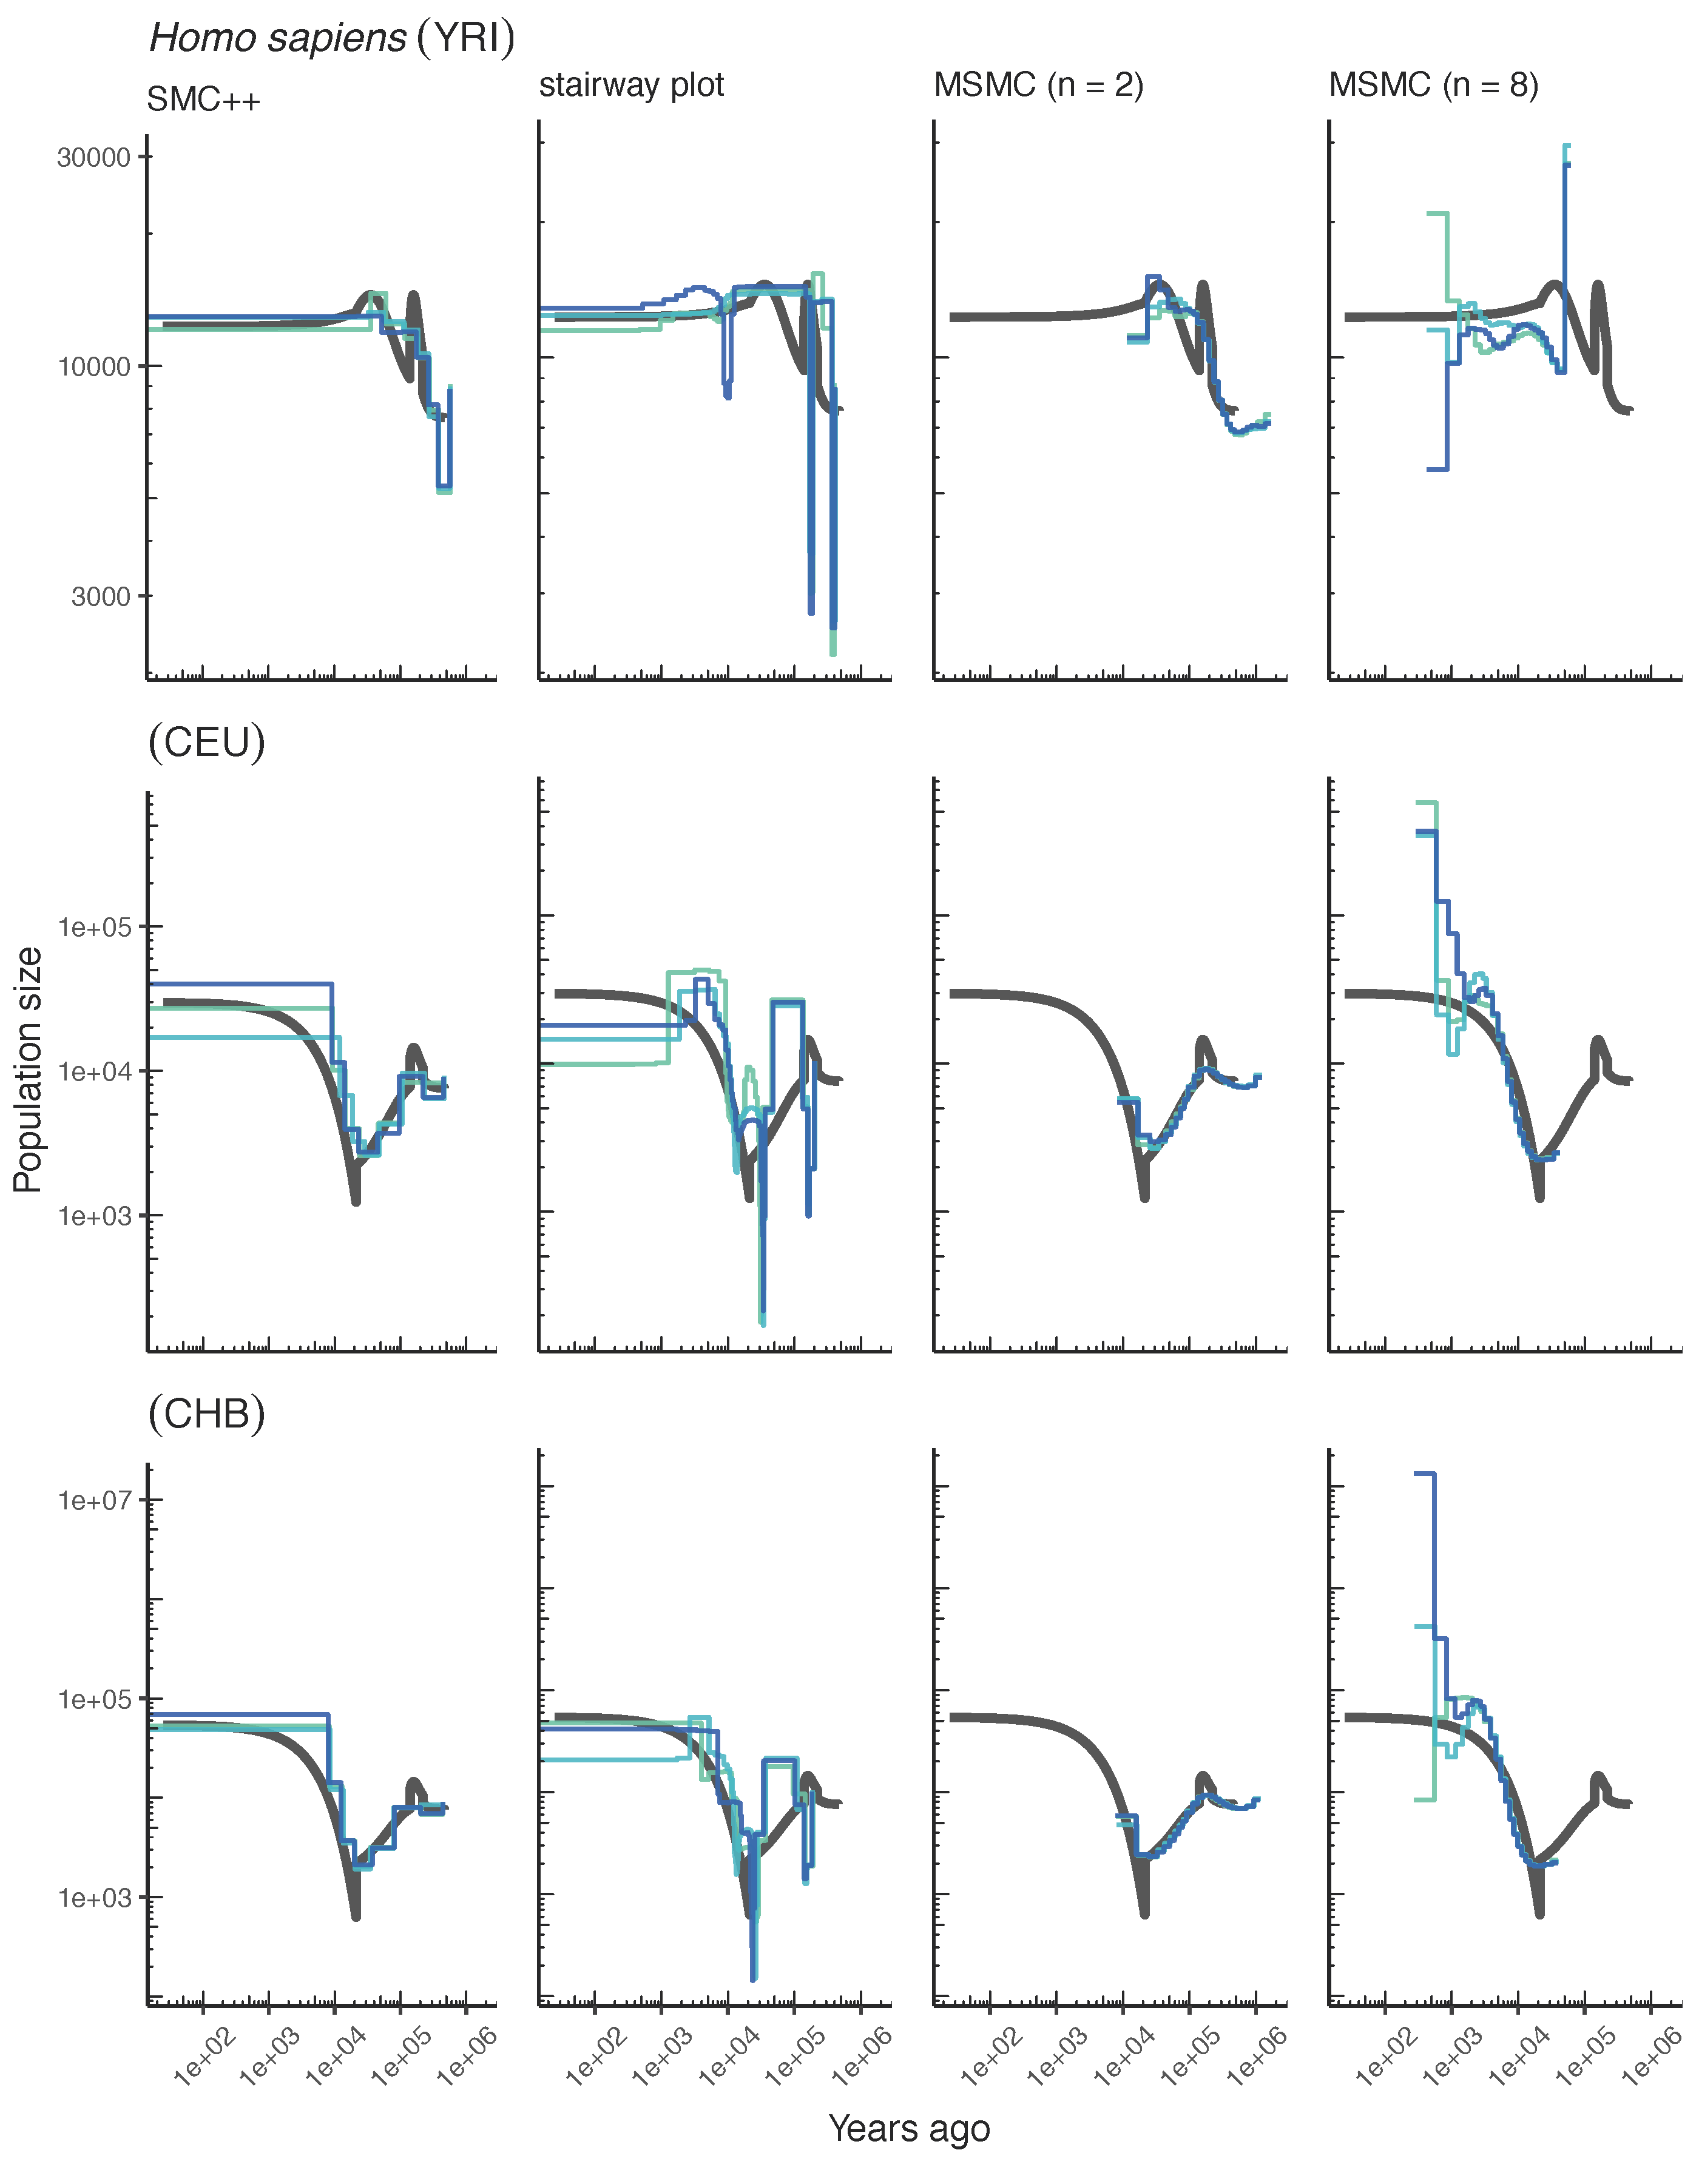
\includegraphics[width=0.8\linewidth]{display_items/homo_sapiens_mask_Gutenkunst.png}
\caption{\textbf{Comparing estimates of $N(t)$ in humans}. Estimates of population
size over time ($N(t)$) inferred using 4 different methods, \smcpp, \stairwayplot, and
\MSMC with $n=2$ and $n=8$. Data were generated by simulating
replicate human genomes under the \cite{gutenkunst2009inferring} model and using the genetic map
inferred in \cite{international2007second}. From top to bottom we show estimates for each
of the three populations in the model: YRI, CEU, and CHB. In shades of blue we show the estimated
$N(t)$ trajectories for each replicate. In black we show the true population size history as inferred
for the rate of coalescence in the demographic model.}
\label{fig:n_t_gutenkunst}
\end{center}
\end{figure}

\begin{figure}
\begin{center}
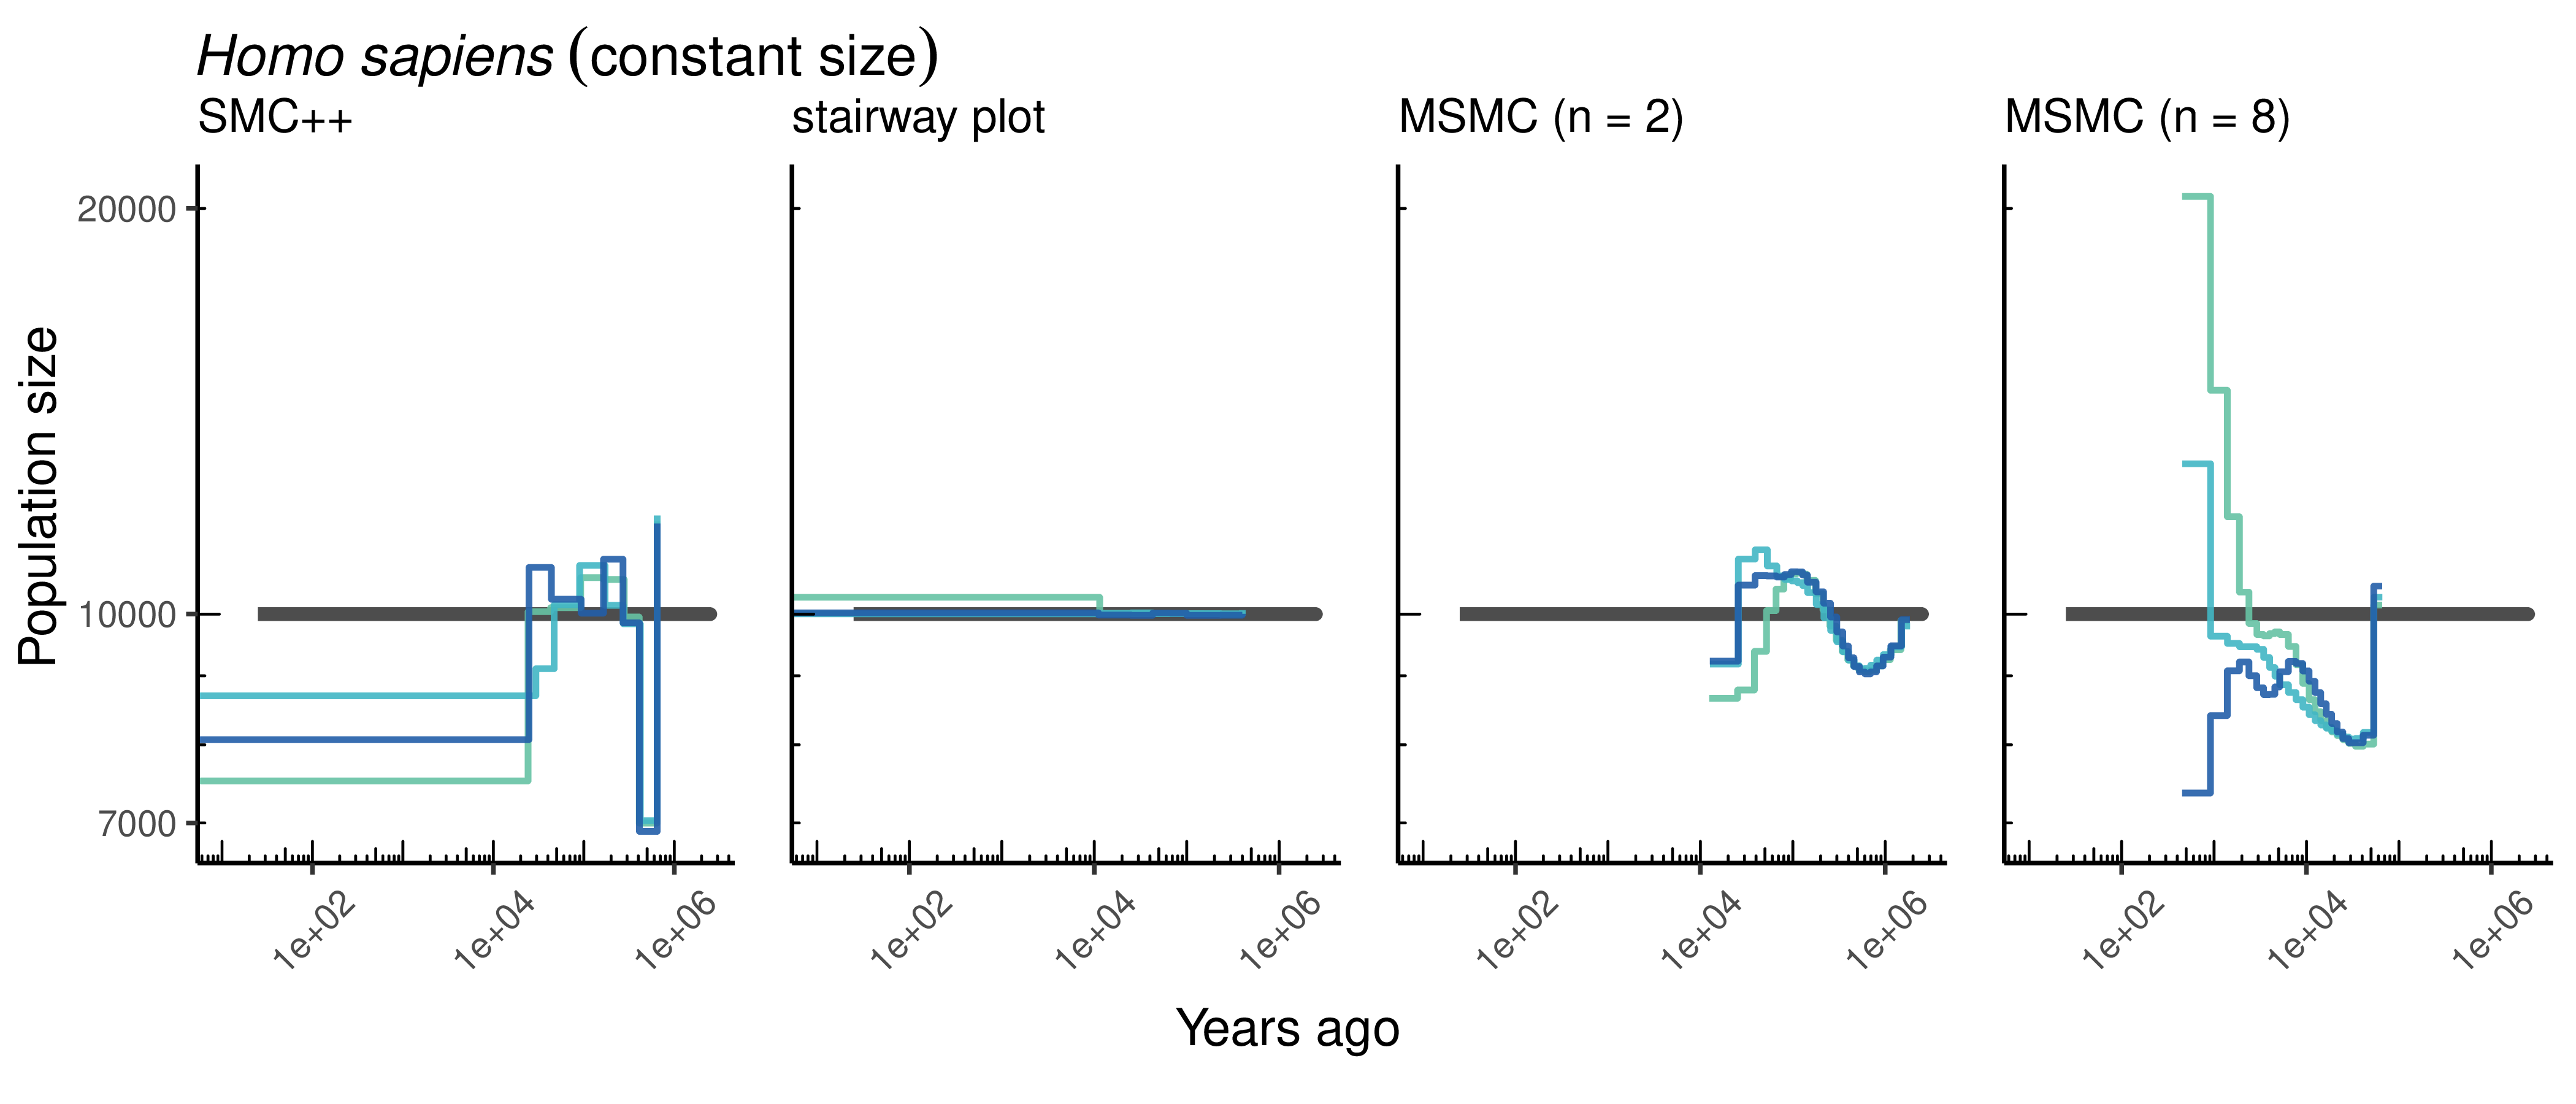
\includegraphics[width=0.8\linewidth]{display_items/homo_sapiens_constant.png}
\caption{\textbf{Comparing estimates of $N(t)$ in humans}. Here we show estimates of population
size over time ($N(t)$) inferred using 4 different methods, \smcpp, and \texttt{stairwayplot},
\MSMC with $n=2$ and $n=8$. Data were generated by simulating
replicate human genomes under a constant sized population model with $N=10^4$ and using the
HapMapII genetic map~\citep{international2007second}. In black we show the true population size history
of the model.}
\label{fig:n_t_HomSap_constant}
\end{center}
\end{figure}


\begin{figure}
\begin{center}
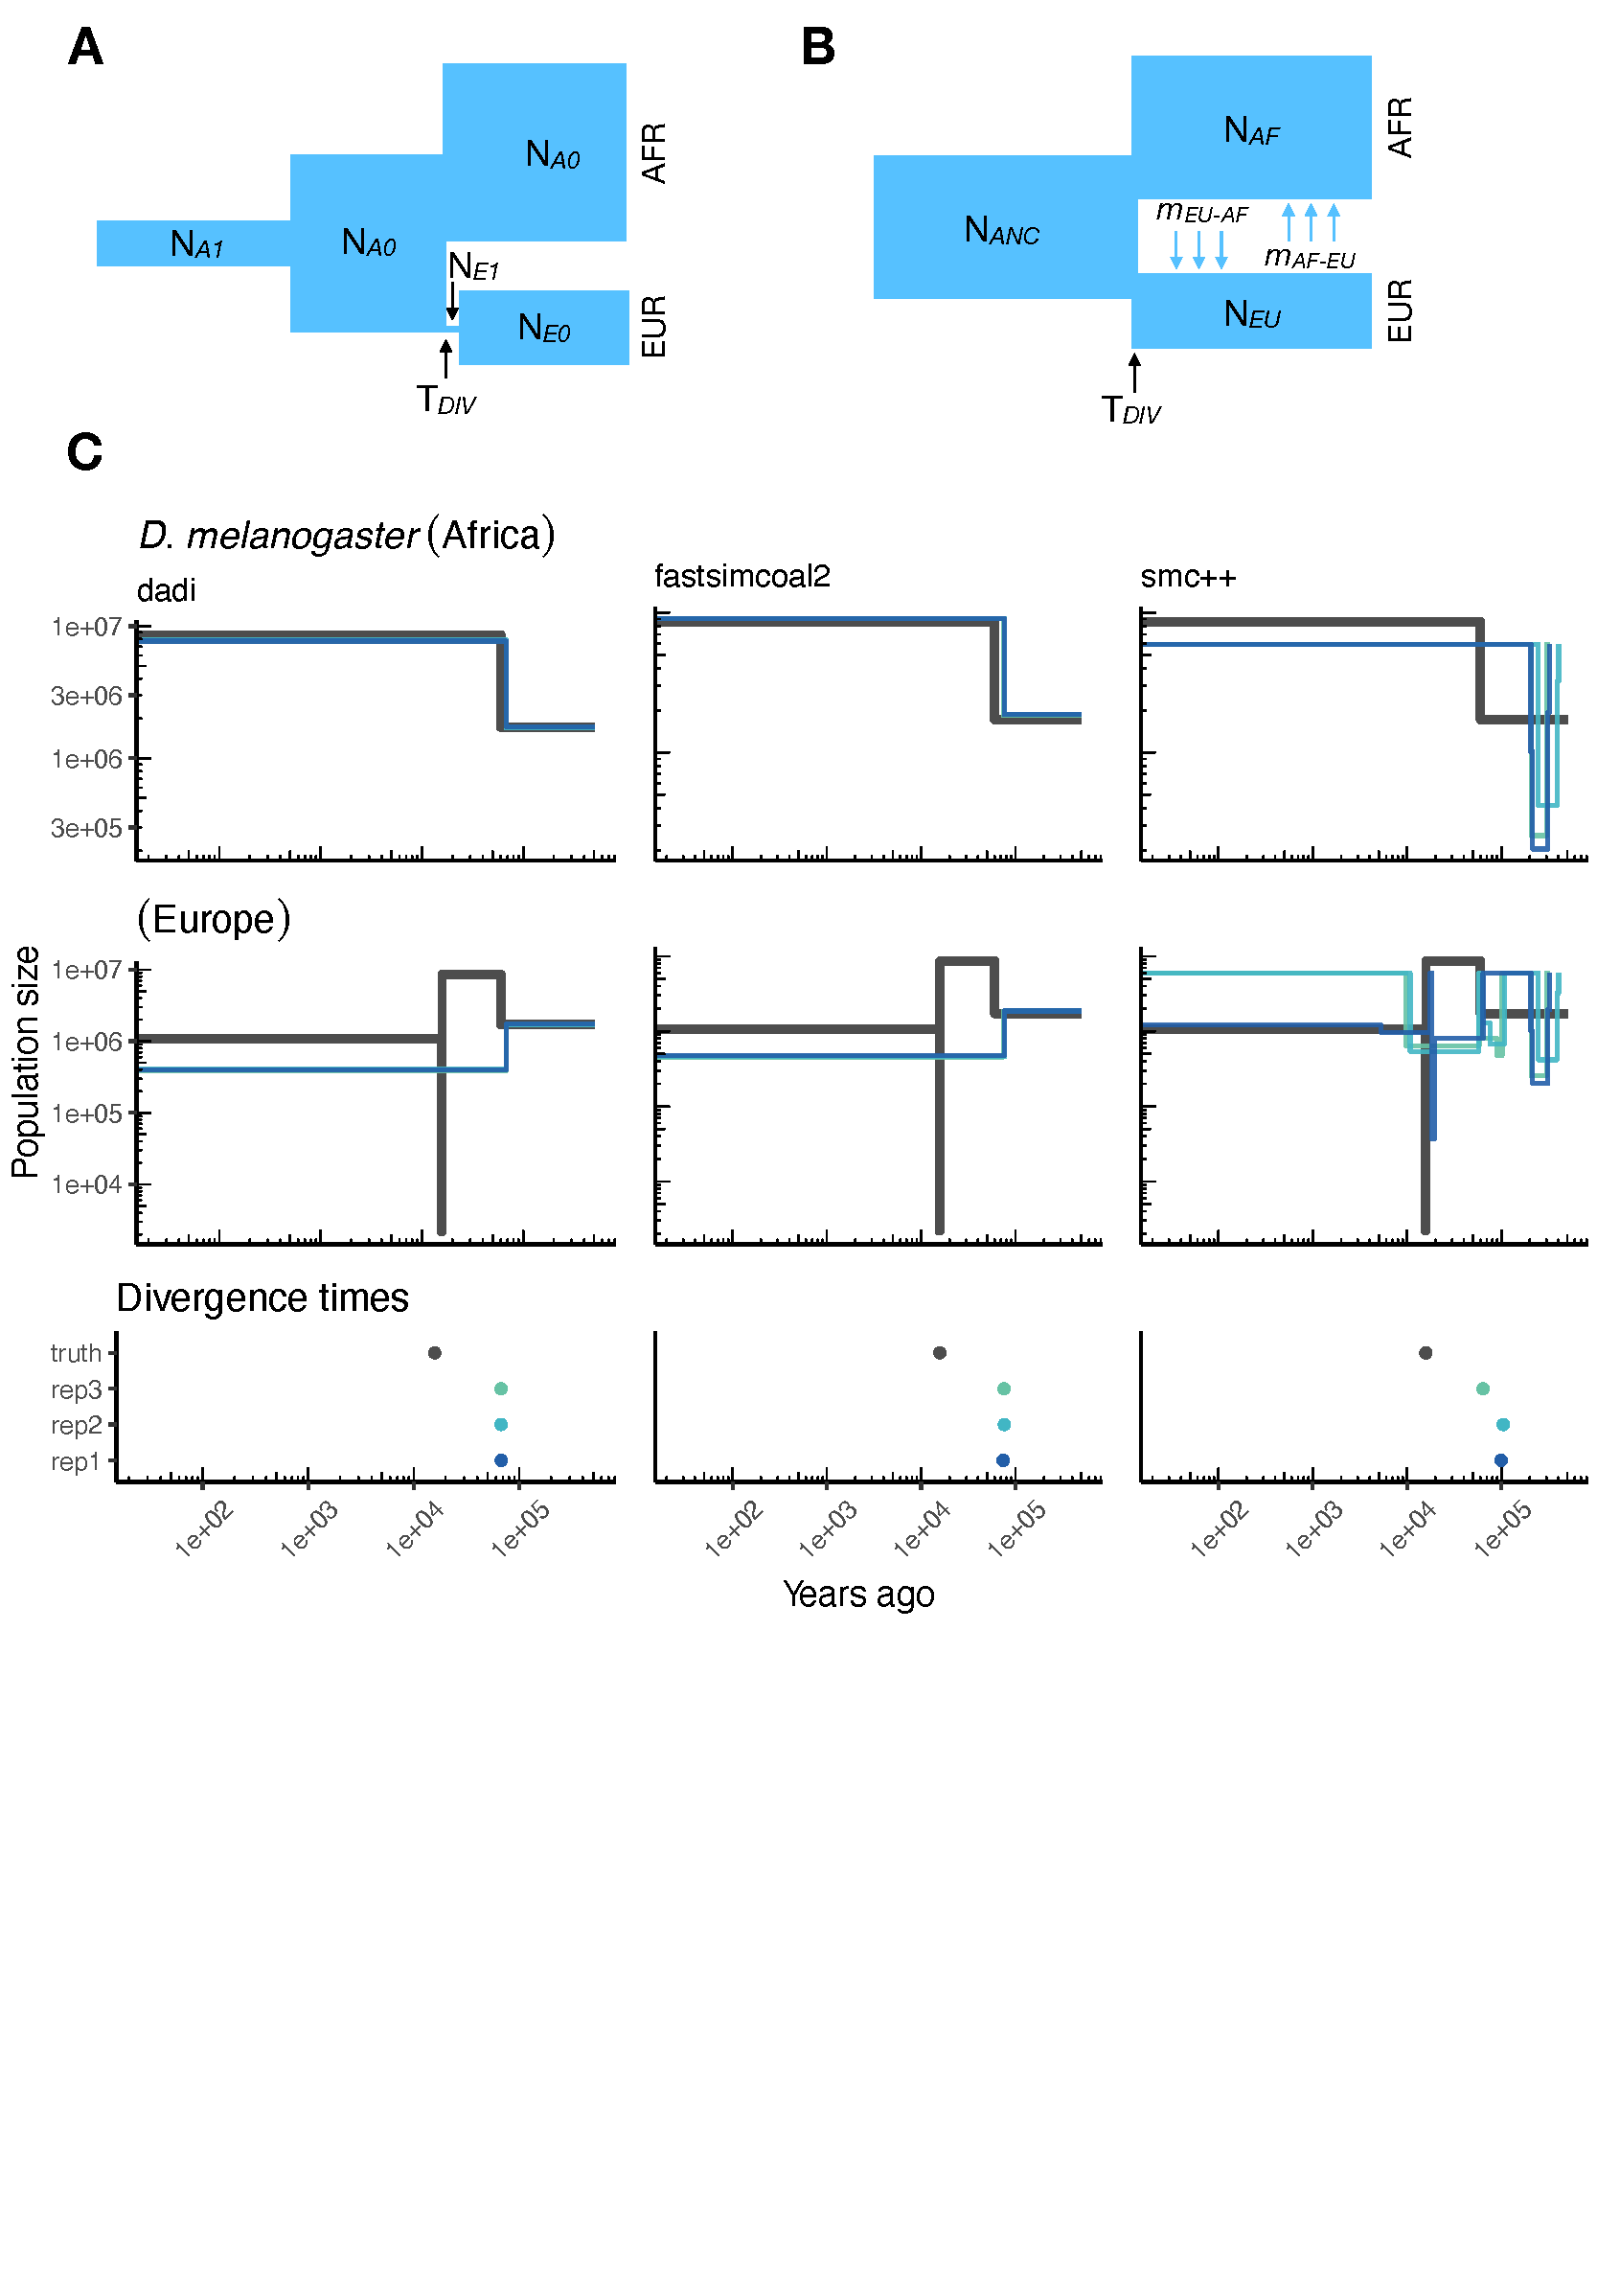
\includegraphics[width=0.8\linewidth]{display_items/d_mel_two_popn_comp.pdf}
\caption{\textbf{Parameters estimated using a two-population \emph{Drosophila} model}.
Here we show estimates of $N(t)$ inferred using \dadi, \fastsimcoal, or \smcpp.
Data were generated by simulating
replicate \emph{Drosophila} genomes under the \cite{li2006inferring} model and using the genetic map
inferred in \cite{comeron2012many}. See legend of Figure \ref{fig:IM_popn_human} for details.
In shades of blue we show the estimated
$N(t)$ trajectories for each replicate. In black we show the true population size history
as given by the census size for the simulated model.}
\label{fig:two_popn_fly}
\end{center}
\end{figure}


\begin{figure}
\begin{center}
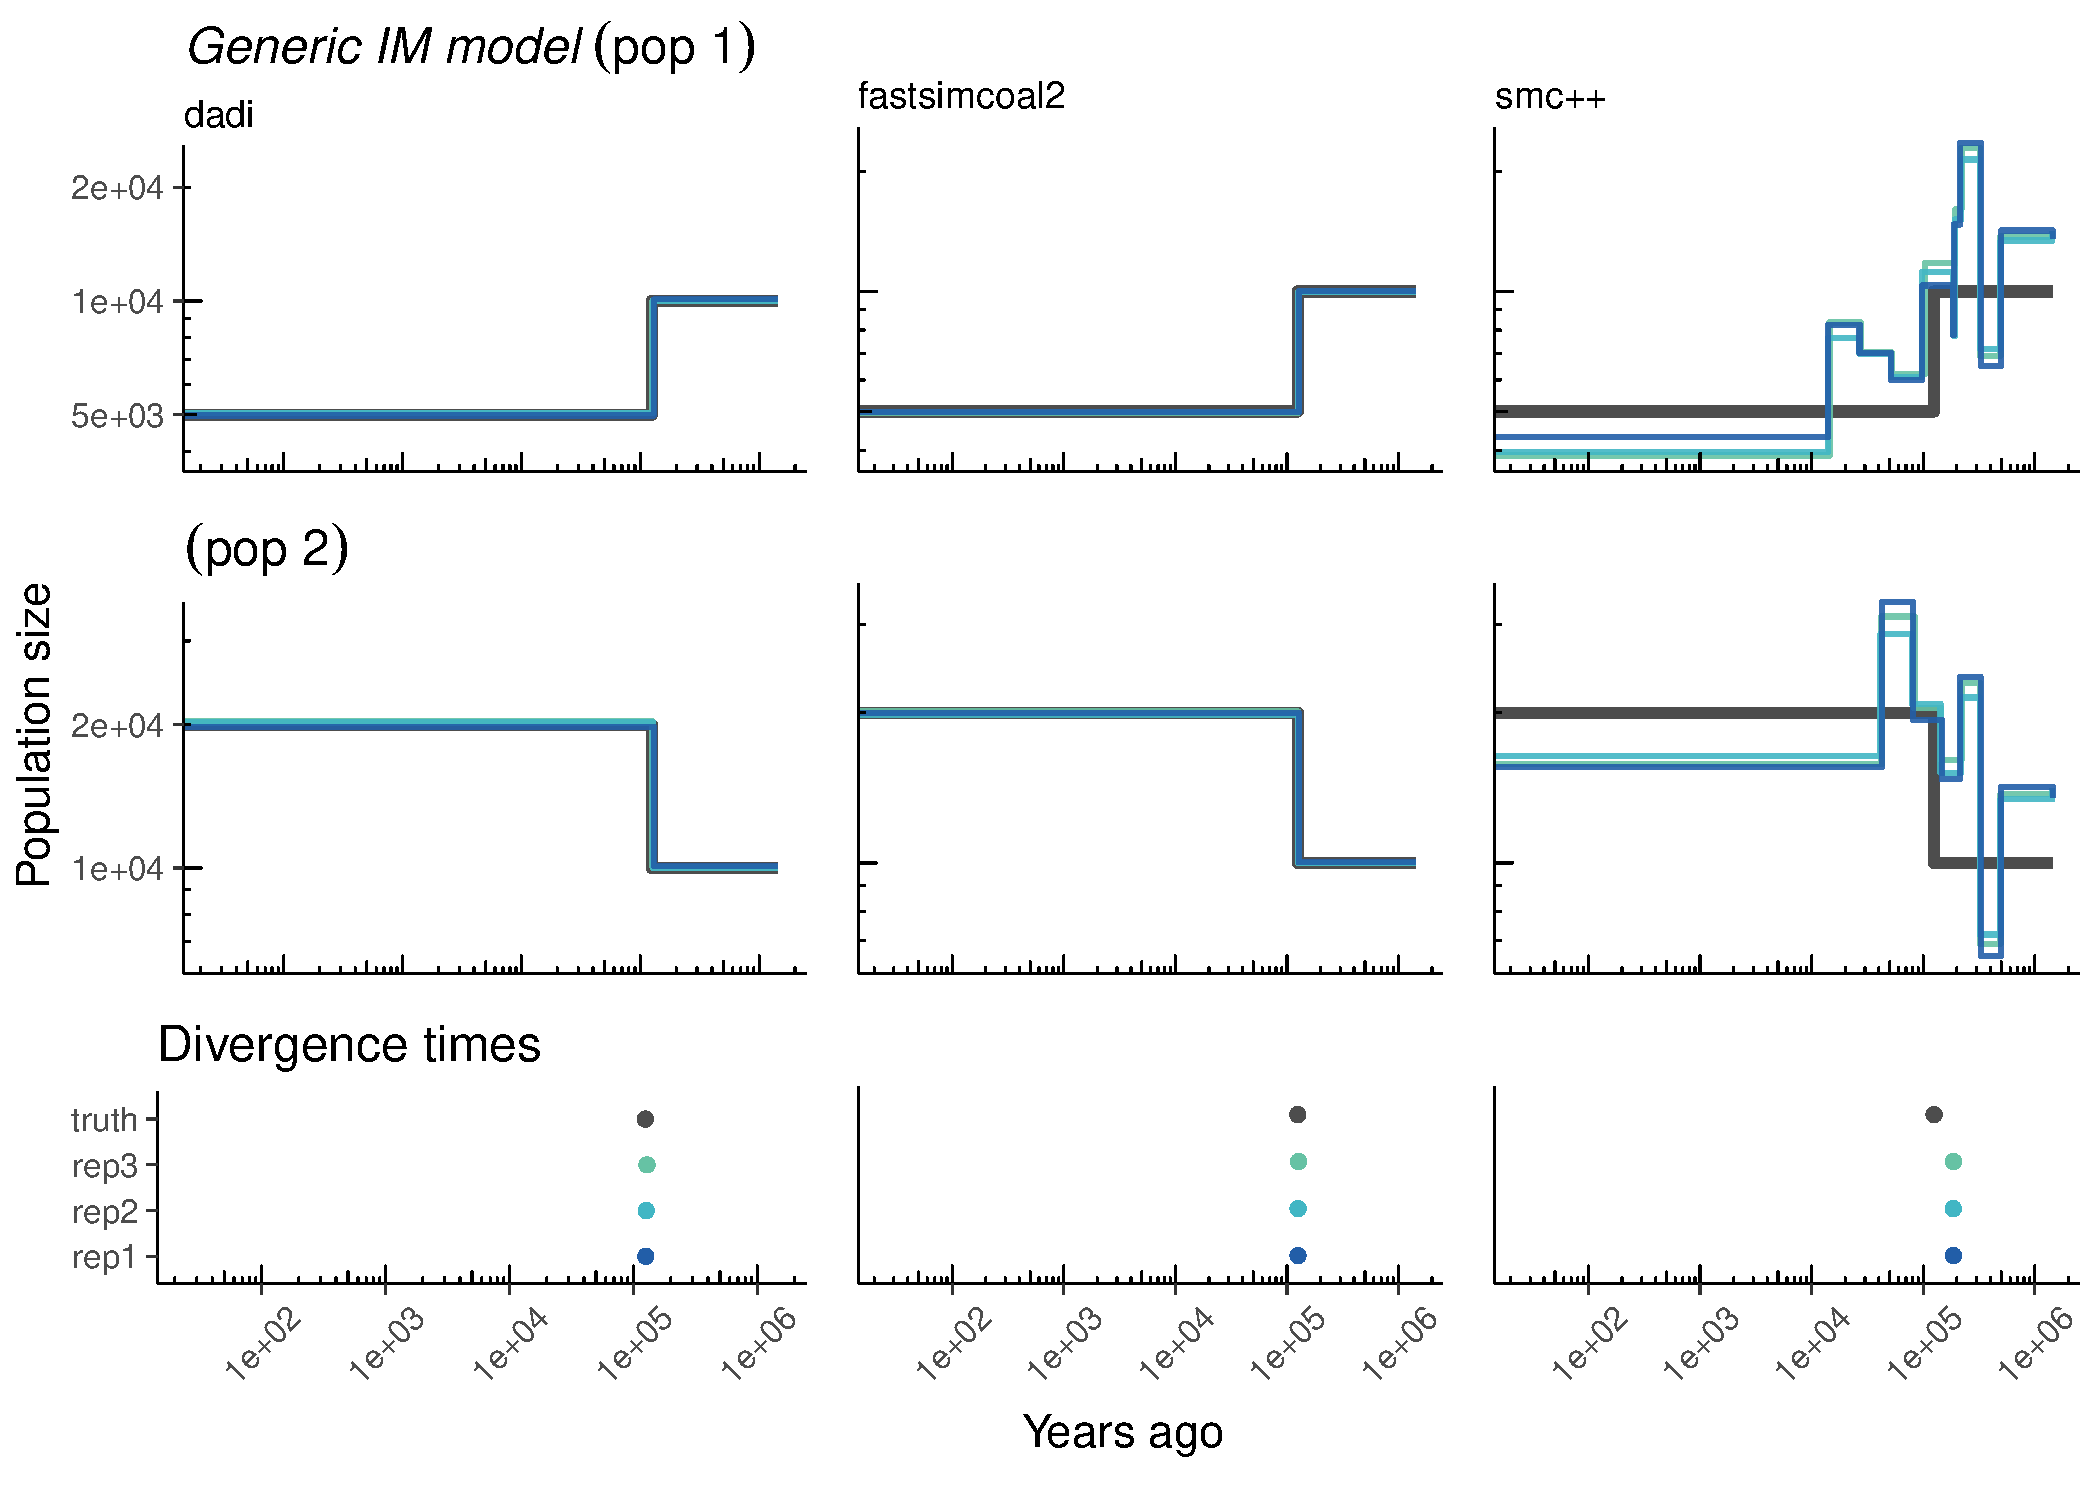
\includegraphics[width=0.8\linewidth]{display_items/generic_IM.pdf}
\caption{\textbf{Parameters estimated from a generic IM model} Here we show estimates of $N(t)$
inferred using \dadi, \texttt{fastsimcoal2}, or \smcpp. Data were generated by simulating
under a generic IM model with a human genome and \cite{international2007second} genetic map.
In shades of blue we show the estimated
$N(t)$ trajectories for each replicate. In black we show the true population size history
as given by the census size for the simulated model.}
\label{fig:generic_IM}
\end{center}
\end{figure}


\begin{figure}
\begin{center}
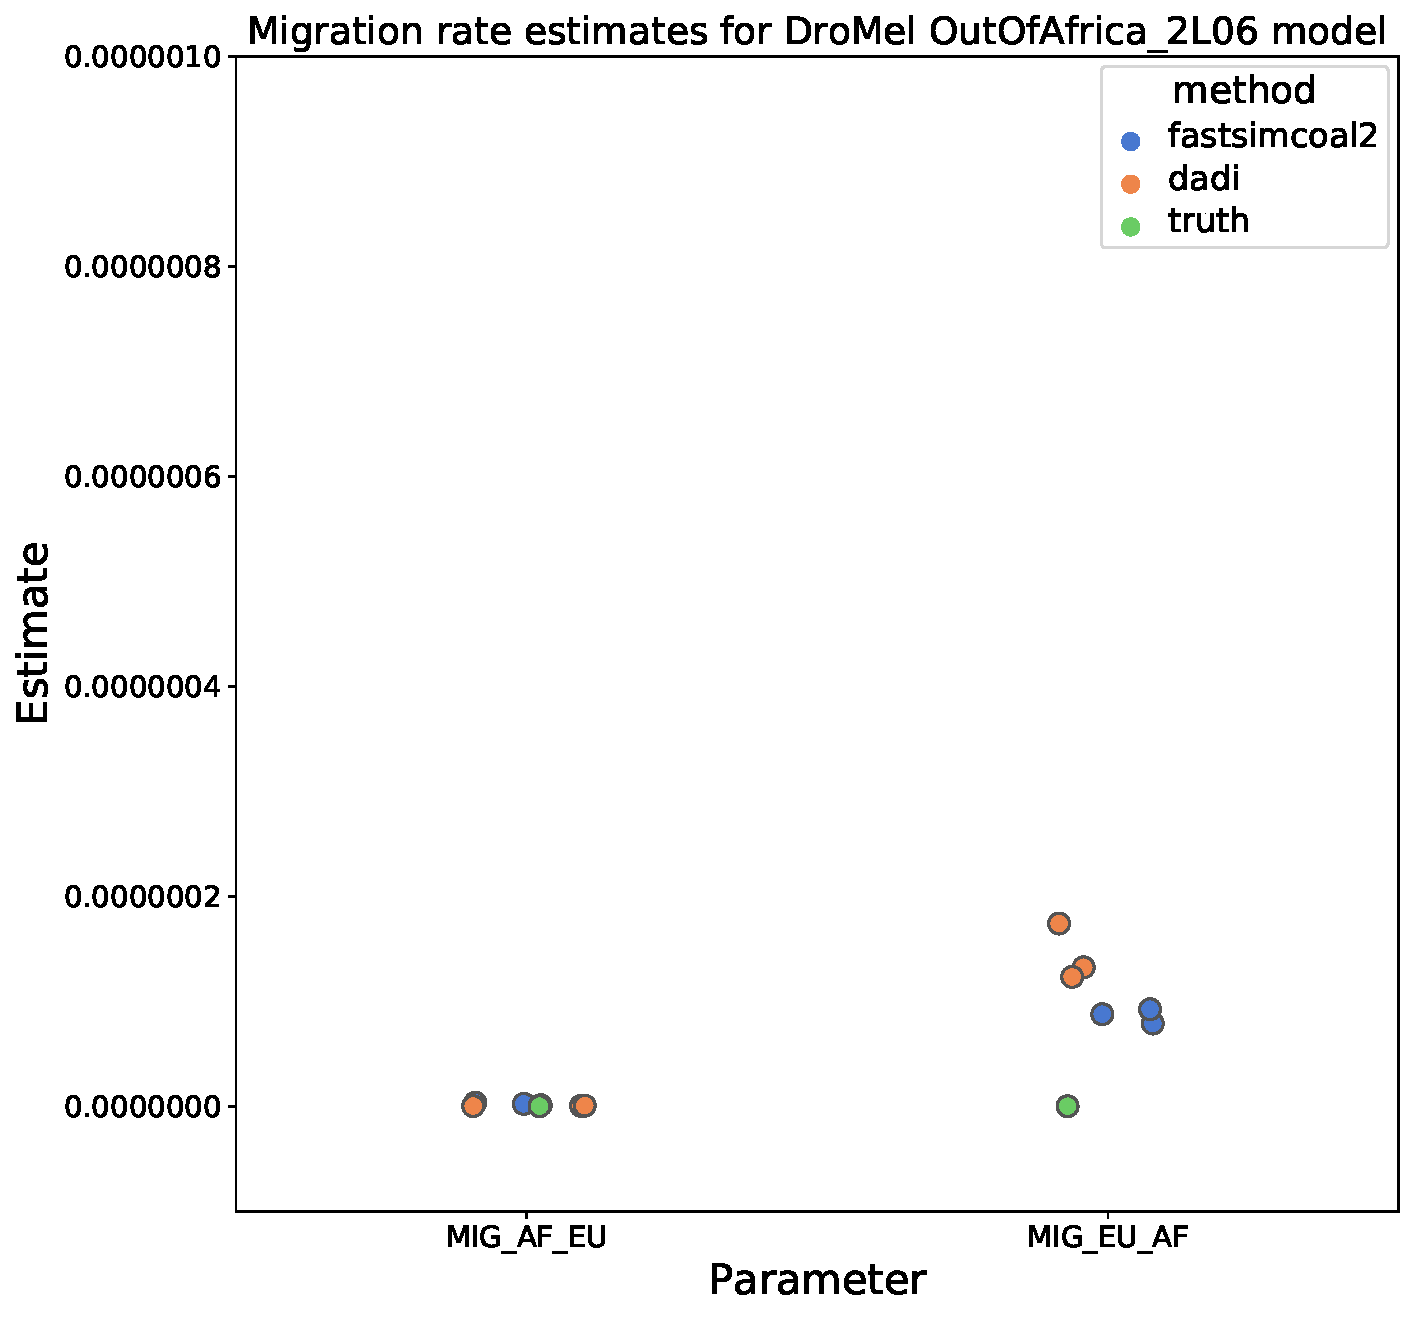
\includegraphics[width=0.8\linewidth]{display_items/dromel_migration_rates.pdf}
\caption{\textbf{Migration rate parameters estimated under a two-population \emph{Drosophila} model}.
Here we show inferred migration rates from \dadi and \fastsimcoal.
Data were generated by simulating replicate \emph{Drosophila} genomes under the \cite{li2006inferring} model and using the genetic map
inferred in \cite{comeron2012many}.}
\label{fig:dromel_mig_rates}
\end{center}
\end{figure}

\begin{figure}
\begin{center}
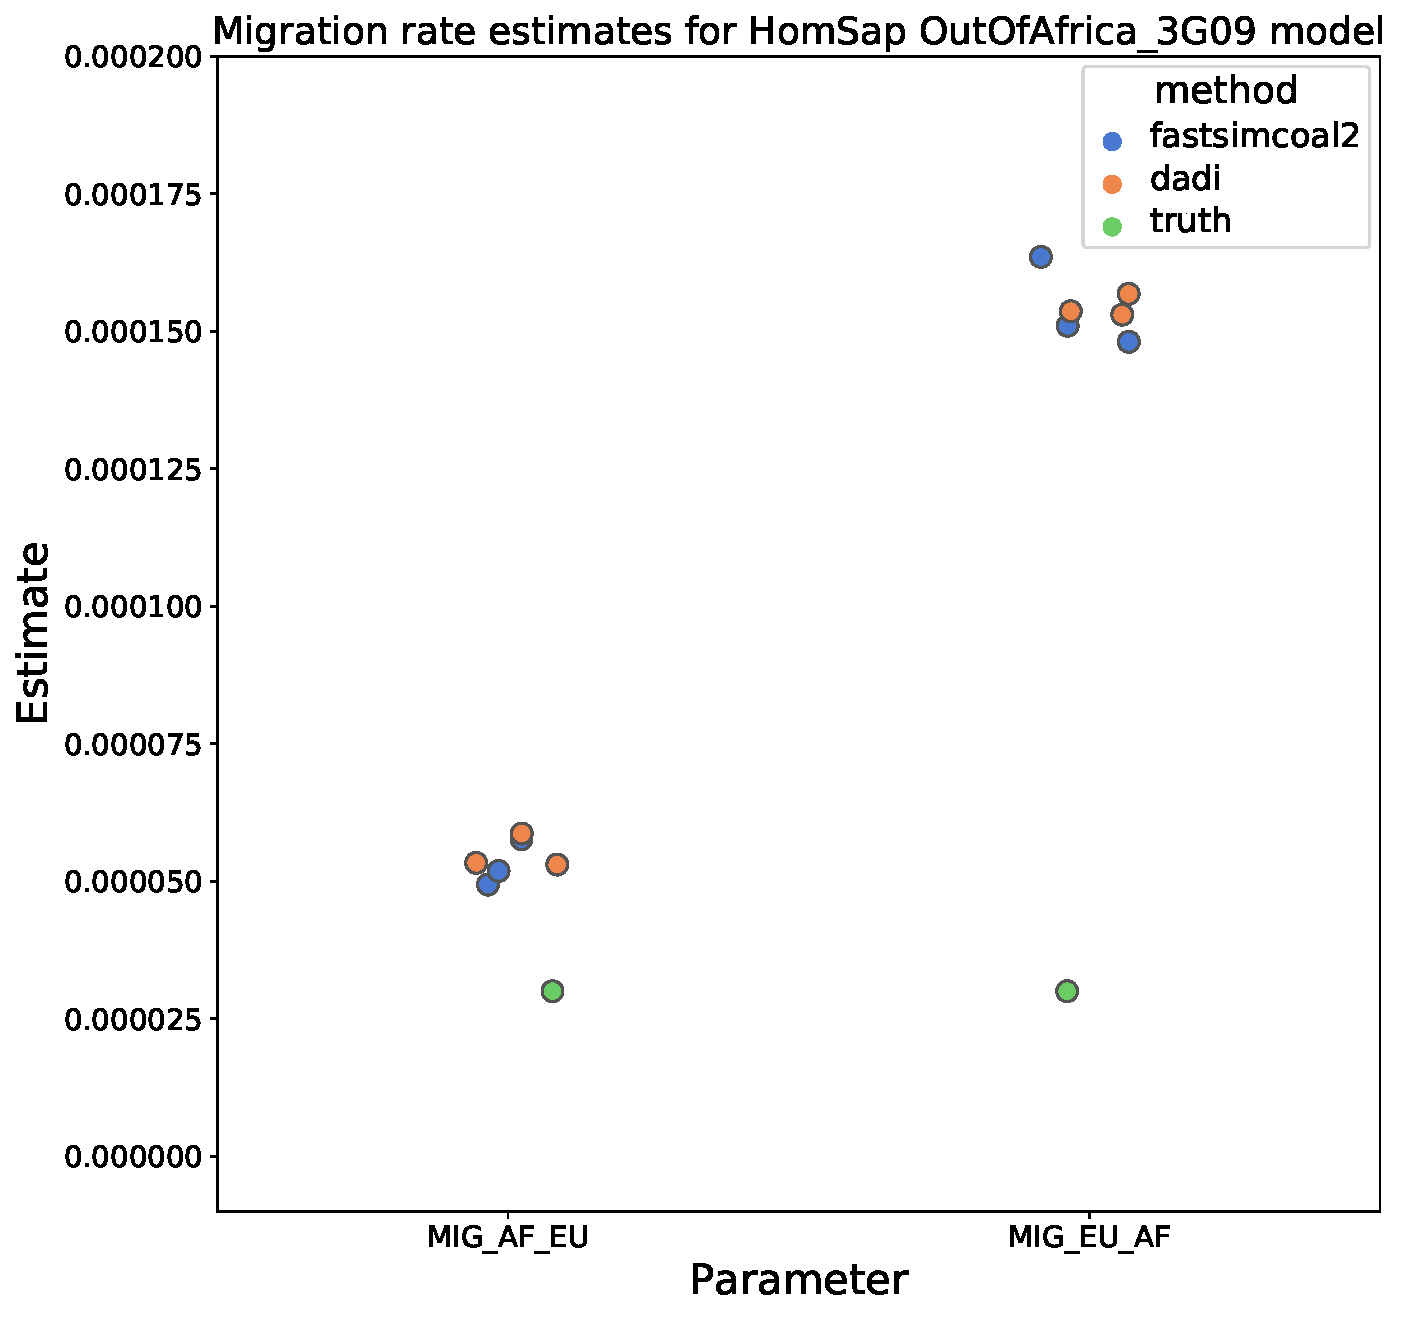
\includegraphics[width=0.8\linewidth]{display_items/homsap_migration_rates.pdf}
\caption{\textbf{Migration rate estimates for the human Gutenkunst model.}
Here we show inferred migration rates from \dadi and \fastsimcoal.
Data were generated by simulating
replicate human genomes under the \cite{gutenkunst2009inferring} model and using the genetic map
inferred in \cite{international2007second}.}
\label{fig:homsap_mig_rates}
\end{center}
\end{figure}


\stopsupplement

\appendix

\section*{Calculating coalescence rates}

We compute the coalescence rate of a collection of samples in a given demographic model
at a particular point back in time
as the expected number of coalescences happening at that time
per unit of time and per pair of as-yet-uncoalesced lineages.
More concretely,
let $p(t)$ denote the probability that the lineages of a randomly chosen pair of samples
have not yet coalesced $t$ units of time ago,
let $p(z, t)$ denote the probability that those lineages have not yet coalesced
and are furthermore both in location $z$,
and let $1/(2 N_e(z,t))$ be the rate of coalescence in location $z$ at the time.
Then, we compute the mean coalescence rate as
$$  r(t)  = \frac{1}{p(t)} \sum_z \frac{p(z,t)}{2N_e(z,t)} . $$
This follows because if we have $n$ diploid samples, and hence $\binom{2n}{2}$ lineages,
the expected number of coalescences in location $z$ between times $t$ and $t+dt$ ago
$$
\binom{2n}{2} p(z,t) \frac{ dt }{ 2 N_e(z,t) },
$$
and the expected number of pairs of uncoalesced lineages at that time is
$$
\binom{2n}{2} p(t) .
$$
The expression for $r(t)$ is a ratio of these two quantities;
to obtain it we need to compute $p(t)$ and $p(z,t)$.
This is relatively straightforward
using the general theory of Markov chains, and is implemented in \texttt{msprime}.

Note that since these quantities are \emph{per pair of lineages},
this definition depends on the locations of the samples.
The coalescence rate also has the intuitive interpretation that
it is the average between-lineage coalescence rate,
averaged over where uncoalesced lineages might be.
Since the local coalescence rate is the inverse of the population size,
$1/r(t)$ (as shown for instance in \autoref{fig:n_t_ragsdale})
is a weighted harmonic mean of the census sizes of the different populations present at that time.
This is as expected: suppose that we have two populations, one big and one small,
connected by migration.
If all our samples are from the big population,
the number of recent coalescences should be small, reflecting the large population size,
while in the long run, the coalescence rate approaches an intermediate rate.
On the other hand, more recent coalescences are expected
if all samples are from the small population,
A method that fits a single, time-varying population size to the data
might be expected to find a population size trajectory
to match these time-varying rates of coalescence.

We use the same computations to analytically compute \emph{mean coalescence times}:
since for any nonnegative random variable $T$, the mean value is
$\mathbb{E}[T] = \int_0^\infty \mathbb{P}\{T > t\} dt$,
we can obtain the mean coalescence time as
$$
\int_0^\infty p(t) dt ,
$$
where $p(t)$ is defined above.

\end{document}
